\documentclass[12pt,a4paper]{article}
% Fix for fancyhdr headheight error
\setlength{\headheight}{14.5pt}
% --- PACKAGES ---
% --- ENCODING & FONTS ---
\usepackage[utf8]{inputenc}
\usepackage[T1]{fontenc}
\usepackage{lmodern}          % Modern font (alternative to Times)
% \usepackage{times}          % OPTIONAL: Classic serif font (comment if using lmodern)

\usepackage{pgf-pie}
\usepackage{pgfplots}
\usepackage{subcaption}
\usepackage{xcolor}
\usepackage{colortbl}
\usepackage{multirow}
\usepackage{booktabs}
\usepackage{siunitx}
\usepackage{float}

% --- PAGE LAYOUT ---
\usepackage[a4paper, left=0.75in, right=0.75in, top=1in, bottom=1in]{geometry}
\usepackage{parskip}          % Paragraphs with spacing instead of indentation
\usepackage{setspace}         % For line spacing

% --- MATHEMATICS ---
\usepackage{amsmath, amsfonts, amssymb}

% --- GRAPHICS & FIGURES ---
\usepackage{graphicx}
\usepackage{caption}
\usepackage{float}
\usepackage{array, longtable, colortbl}
\usepackage{tabularx}

% --- COLORS ---
\usepackage[table]{xcolor}
\usepackage{xcolor}           % General color usage

% --- TIKZ & DIAGRAMS ---
\usepackage{tikz}
\usetikzlibrary{
  shapes.geometric,
  arrows.meta,
  positioning,
  fit,
  backgrounds,
  shapes.multipart
}

% --- PLOTS & CHARTS ---
\usepackage{pgf-pie}          % Pie charts
\usepackage{pgfplots}         % Graphs and plots
% Set pgfplots compatibility for modern features
\pgfplotsset{compat=1.18}

% --- DOCUMENT STRUCTURE ---
\usepackage{titlesec}         % Custom section titles
\usepackage{tocloft}          % Table of contents formatting
\usepackage{enumitem}         % Better lists

% --- HEADER, FOOTER & LINKS ---
\usepackage{fancyhdr}         % Custom headers/footers

% --- BIBLIOGRAPHY ---
\usepackage[numbers,sort&compress]{natbib}  % For references with numerical citations
\bibliographystyle{plainnat}  % Compatible style with natbib
\usepackage[many]{tcolorbox}
\tcbuselibrary{skins,breakable}

% --- Code listings for source code in Appendix ---
\usepackage{listings}
\lstset{
    language=Python,
    basicstyle=\ttfamily\small,
    breaklines=true,
    showstringspaces=false,
    numbers=left,
    numberstyle=\tiny\color{gray},
    frame=single,
    captionpos=b,
    keywordstyle=\color{blue},
    commentstyle=\color{green!60!black},
    stringstyle=\color{purple},
    rulecolor=\color{black!20},
    backgroundcolor=\color{black!5}
}

% --- Load hyperref last ---
\usepackage{hyperref}         % Clickable links


% --- COLORS ---
\definecolor{RoyalBlue}{RGB}{0, 70, 140}
\definecolor{RUETRed}{RGB}{179, 0, 0}
\definecolor{LightGray}{RGB}{248, 249, 250}
\definecolor{DarkGray}{RGB}{52, 58, 64}
\definecolor{AccentBlue}{RGB}{13, 110, 253}
\definecolor{ModernGray}{RGB}{108, 117, 125}
\definecolor{lightgreen}{RGB}{200, 255, 200}
\definecolor{lightred}{RGB}{255, 200, 200}

% Define modern color palette
\definecolor{primary}{RGB}{41, 128, 185}
\definecolor{secondary}{RGB}{52, 152, 219}
\definecolor{accent}{RGB}{231, 76, 60}
\definecolor{success}{RGB}{46, 204, 113}
\definecolor{warning}{RGB}{241, 196, 15}
\definecolor{darkgray}{RGB}{52, 73, 94}
\definecolor{lightgray}{RGB}{236, 240, 241}
\definecolor{purple}{RGB}{155, 89, 182}
\definecolor{orange}{RGB}{230, 126, 34}
\definecolor{teal}{RGB}{26, 188, 156}
\definecolor{OliveGreen}{RGB}{85, 107, 47}

\definecolor{outputbg}{RGB}{45, 45, 45} % Dark background for output

% --> ADDED for the blue info box
% --> Define colors for code boxes and result boxes
\definecolor{reportgreen}{RGB}{230, 245, 230}
\definecolor{reportdarkgreen}{RGB}{50, 120, 50}
\definecolor{outputbg}{RGB}{45, 45, 45} % Dark background for output
\definecolor{infoboxbg}{RGB}{235, 245, 255}
\definecolor{infoboxborder}{RGB}{70, 130, 180}
% --> ADDED: Define the blue info box style
\newtcolorbox{infobox}{
  colback=infoboxbg,
  colframe=infoboxborder,
  boxrule=0.5pt, % thin border for sides/bottom
  borderline north={1.5pt}{0pt}{infoboxborder}, % thicker top border
  arc=0mm,       % sharp corners
  left=5mm, % Add some padding
  top=3mm,
  bottom=3mm
}

% --> Define style for code listings (like Listing 2, 3 in friend's report)
\lstdefinestyle{code}{
    basicstyle=\ttfamily\small,
    numbers=left,
    numberstyle=\tiny\color{gray},
    numbersep=5pt,
    frame=none,
    breaklines=true,
    keywordstyle=\color{blue},
    commentstyle=\color{OliveGreen},
    stringstyle=\color{purple},
    showstringspaces=false
}
\lstset{style=code} % Set default listing style

% --> Define the green result box
\newtcolorbox{resultbox}[2][]{
    enhanced,
    attach boxed title to top center={yshift=-2mm},
    colback=reportgreen,
    colframe=reportdarkgreen,
    colbacktitle=reportgreen,
    coltitle=black,
    boxed title style={size=small,colframe=reportdarkgreen},
    title={#2},
    fonttitle=\bfseries
}

% --- FONT & STYLING ---
\renewcommand{\familydefault}{\sfdefault}  % Use sans-serif font
\titleformat{\section}{\fontsize{20}{24}\selectfont\bfseries\color{RoyalBlue}}{\thesection}{1em}{}
\titleformat{\subsection}{\fontsize{16}{20}\selectfont\bfseries\color{RoyalBlue}}{\thesubsection}{1em}{}
\titleformat{\subsubsection}{\fontsize{13}{16}\selectfont\bfseries\color{RoyalBlue}}{\thesubsubsection}{1em}{}

% TOC Styling
\renewcommand{\cfttoctitlefont}{\color{black}\Huge\bfseries}
\renewcommand{\cftsecfont}{\color{RoyalBlue}}
\renewcommand{\cftsecpagefont}{\color{RoyalBlue}}
\renewcommand{\cftsubsecfont}{\color{RoyalBlue}}
\renewcommand{\cftsubsecpagefont}{\color{RoyalBlue}}

% Header and Footer
\pagestyle{fancy}
\fancyhf{}
\fancyhead[C]{\textit{Data Mining Report}}
\fancyfoot[C]{\thepage}
\renewcommand{\headrulewidth}{0.4pt}
\renewcommand{\footrulewidth}{0pt}

% Hyperlink Styling
\hypersetup{
    colorlinks=true,
    linkcolor=RoyalBlue,
    filecolor=magenta,
    urlcolor=cyan,
    pdftitle={Data Mining Report},
    pdfpagemode=FullScreen,
    pdfborder={0 0 0},
}

% --- Define a global style for all plots for consistency ---
\pgfplotsset{
    every axis/.append style={
        axis x line=bottom,
        axis y line=left,
        label style={font=\bfseries},
        title style={font=\large\bfseries, yshift=1em},
        tick label style={font=\small},
        legend style={font=\small, at={(0.5,-0.2)}, anchor=north, legend columns=-1},
    }
}

% Modern title page with geometric design
\newcommand{\maketitlepage}{
    \begin{titlepage}
        \begin{tikzpicture}[remember picture,overlay]
            \fill[RoyalBlue!10] (current page.north west) rectangle ([yshift=-2.2cm]current page.north east);
            \fill[AccentBlue!5] ([yshift=-14cm]current page.north west) rectangle ([yshift=-16.2cm]current page.north east);
            \fill[RoyalBlue!15] ([xshift=2cm,yshift=-2cm]current page.north west) circle (1.2cm);
            \fill[AccentBlue!15] ([xshift=-2cm,yshift=-15.2cm]current page.north east) circle (0.9cm);
        \end{tikzpicture}

        \centering
        \vspace*{0.6cm}

        % Logo (only include if file exists)
        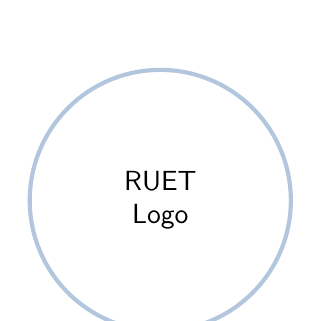
\begin{tikzpicture}
            \node[circle, draw=RoyalBlue!30, line width=1.5pt, inner sep=6pt] at (0,0) {
                 \IfFileExists{RUET_logo.png}{\includegraphics[width=2.7cm]{RUET_logo.png}}{\begin{minipage}{2.7cm}\centering RUET \\ Logo \end{minipage}}
            };
        \end{tikzpicture}

        \vspace{0.6cm}
        {\fontsize{15.5}{17}\selectfont\bfseries\textcolor{RUETRed}{RAJSHAHI UNIVERSITY OF ENGINEERING \& TECHNOLOGY}\par}
        \vspace{0.2cm}
        {\fontsize{13.5}{16}\selectfont\textcolor{DarkGray}{Department of Computer Science and Engineering}\par}

        \vspace{1.5cm}
        % Title Block
        
\begin{tikzpicture}
            \node[rectangle, fill=RoyalBlue!5, rounded corners=12pt, inner sep=12pt, text width=11.5cm, align=center] at (0,0) {
                {\fontsize{21}{24}\selectfont\bfseries\textcolor{RoyalBlue}{LAB REPORT}\par}
                \vspace{0.15cm}
                {\fontsize{16}{20}\selectfont\bfseries\textcolor{DarkGray}{-}\par}
                \vspace{0.15cm}
                {\fontsize{24}{28}\selectfont\bfseries\textcolor{AccentBlue}{"DATA MINING"}\par}
            };
        \end{tikzpicture}

        \vspace{1.8cm}
        % Submission info
        \begin{minipage}[t]{0.45\textwidth}
            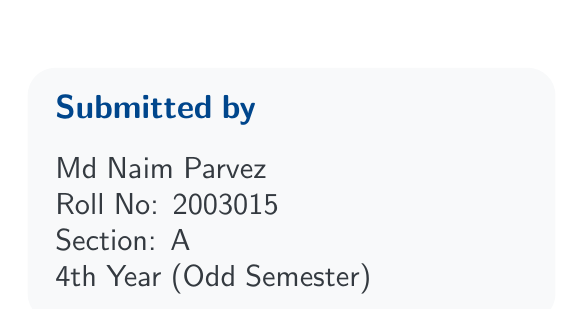
\begin{tikzpicture}
                \node[rectangle, fill=LightGray, rounded corners=10pt, inner sep=10pt, text width=6cm] at (0,0) {
                    {\fontsize{13}{15}\selectfont\bfseries\textcolor{RoyalBlue}{Submitted by}\par}
                    \vspace{0.3cm}
                    {\fontsize{11}{13}\selectfont\textcolor{DarkGray}{
                        Md Naim Parvez\\
                        Roll No: 2003015\\
                        Section: A\\
                        4th Year (Odd Semester)
                    }\par}
                };
            \end{tikzpicture}
        \end{minipage}
        \hfill
        \begin{minipage}[t]{0.50\textwidth}
            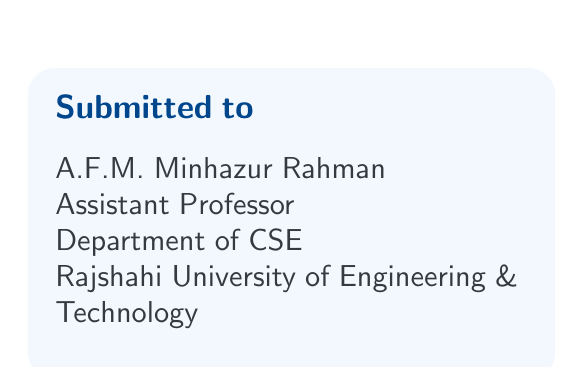
\begin{tikzpicture}
                \node[rectangle, fill=AccentBlue!5, rounded corners=10pt, inner sep=10pt, text width=6cm] at (0,0) {
                    {\fontsize{13}{15}\selectfont\bfseries\textcolor{RoyalBlue}{Submitted to}\par}
                    \vspace{0.3cm}
                    {\fontsize{11}{13}\selectfont\textcolor{DarkGray}{
                        A.F.M. Minhazur Rahman\\
                        Assistant Professor\\
                        Department of CSE\\
                        Rajshahi University of Engineering \& Technology\\
                        \vspace{0.3cm}
                    }\par}
                };
            \end{tikzpicture}
        \end{minipage}

        \vspace{1.2cm}
        % Course Info
        
\begin{tikzpicture}
            \node[rectangle, fill=RoyalBlue!10, rounded corners=10pt, inner sep=12pt, align=center, text width=13cm] at (0,0) {
                {\fontsize{13}{16}\selectfont\bfseries\textcolor{RoyalBlue}{Course Code: } \textcolor{DarkGray}{4120}}\\[0.2cm]
                {\fontsize{13}{16}\selectfont\bfseries\textcolor{RoyalBlue}{Course Title: } \textcolor{DarkGray}{Data Mining Sessional}}
            };
        \end{tikzpicture}

        \vspace{0.8cm}
    \end{titlepage}
}


\begin{document}

% --- TITLE PAGE ---
\maketitlepage
\thispagestyle{empty} % No header/footer on the title page

\newpage
% --- TABLE OF CONTENTS ---
\pagenumbering{roman} % Roman numerals for ToC, Abstract etc.
\phantomsection % Helps hyperref create proper links
\tableofcontents

% --- LIST OF FIGURES ---
\newpage
\phantomsection % Helps hyperref create proper links
\listoffigures
\newpage
\pagenumbering{arabic} % Arabic numerals for main content
\setcounter{page}{1} % Start main content page numbering from 1


%----------------------------------------------------------
% 1. Introduction
%----------------------------------------------------------
\section{Introduction}

\subsection{Motivation and Dataset Selection}

Road safety is a critical global concern, with traffic accidents ranking among the leading causes of injury and death worldwide. Identifying and predicting high-risk road conditions are essential steps toward designing smarter transportation systems and saving lives.  

For this project, the \textbf{Road Accident Risk Dataset} was selected. This synthetic dataset simulates real-world road conditions and represents a diverse range of environmental, infrastructural, and temporal variables. Its design supports predictive modeling tasks focused on estimating accident probabilities across different road segments.

\begin{infobox}{}
\textbf{Why Road Accident Risk Dataset?}
\begin{itemize}
    \item \textit{Real-World Context:} The dataset reflects the multidimensional nature of traffic safety—weather, lighting, surface type, and traffic density all interact to determine risk.
    \item \textit{Classification Feasibility:} By categorizing segments into low-, medium-, and high-risk classes, supervised learning algorithms can be effectively applied.
    \item \textit{Clustering Potential:} Numerical and categorical features allow for unsupervised exploration to uncover natural accident patterns.
    \item \textit{Data Challenge:} The dataset includes missing values and simulated anomalies, providing an opportunity to develop robust preprocessing pipelines.
\end{itemize}
\vspace{1cm}
The dataset was sourced from an active Kaggle competition, providing an opportunity to benchmark solutions against the data science community. The dataset can be accessed at: \url{https://www.kaggle.com/competitions/playground-series-s5e10/data}.
\end{infobox}

\subsection{Lab Objectives and Task Overview}

The work follows a multi-stage data mining pipeline, composing tasks that transform raw data into actionable insights:

\begin{enumerate}
    \item \textit{Lab 1 – Dataset Analysis:}Understanding data structure, dimensions, and classification problem formulation. This initial step is crucial for identifying data types, detecting potential issues early, and determining the appropriate machine learning approach before investing time in modeling
    \item \textit{Lab 2 – Data Preprocessing:} Handling missing values, outliers, encoding, scaling, and similarity measures. Preprocessing is essential because algorithms cannot handle missing data or categorical variables directly, and unscaled features can bias distance-based methods.Quality input ensures quality output.
    \item \textit{Lab 3 – Exploratory Data Analysis (EDA):} Visualizing distributions, correlations, and patterns within the dataset. EDA provides insights into feature importance, class imbalances, and potential relationships that inform model selection and feature engineering strategies.
    \item \textit{Lab 4 – Mining Frequent Itemsets:} Applying Apriori/FP-Growth algorithm to discover frequent patterns and association rules. Analysis of support, confidence, and lift metrics reveals purchase behaviors and product relationships. Understanding these patterns helps optimize inventory management and marketing strategies.
    \item \textit{Lab 5 – Classification:} Building Decision Tree models with entropy and Gini criteria.Classification transforms our understanding into actionable predictions, allowing us to automatically categorize fuel efficiency. Comparing criteria helps us select the optimal splitting strategy.
    \item \textit{Lab 6 – Clustering:} Applying k-Means and hierarchical clustering to discover natural groupings. Clustering uncovers hidden vehicle segments without predefined labels, validating our classification approach and revealing market structures that might inform manufacturing or marketing strategies.
\end{enumerate}

\begin{infobox}
\textbf{Why These Tasks Are Important:}
Each stage builds logically upon the previous one. Preprocessing ensures data quality; EDA uncovers structure and guides model selection; classification predicts accident risk levels; clustering validates hidden patterns. Together, they demonstrate how data-driven insights can translate into safer roads and informed infrastructure planning.
\end{infobox}
\section{Lab Tasks and Implementation}

\subsection{Lab 1: Dataset Analysis}

\subsubsection{Initial Data Loading and Inspection}
\begin{lstlisting}[language=Python]
df_train = pd.read_csv('train.csv')
df_train = df_train.head(1000).reset_index(drop=True).copy()
df_train.drop(['id','num_lanes','time_of_day'],axis=1,inplace=True)
print("--- Task 1.1: Data Dimensions ---")
print(f"The dataset has {df_train.shape[0]} rows and {df_train.shape[1]} columns.")

print("--- Task 1.2: Data Types and Info ---")
# This command prints the data types, non-null counts, and memory usage.
# This is the MOST IMPORTANT output for this lab.
df_train.info()
print("\n")

print("--- Task 1.3: First 5 Rows (to help find label) ---")
# This helps you visually inspect the columns
df_train.head()
\end{lstlisting}

\begin{figure}[H]
    \centering
    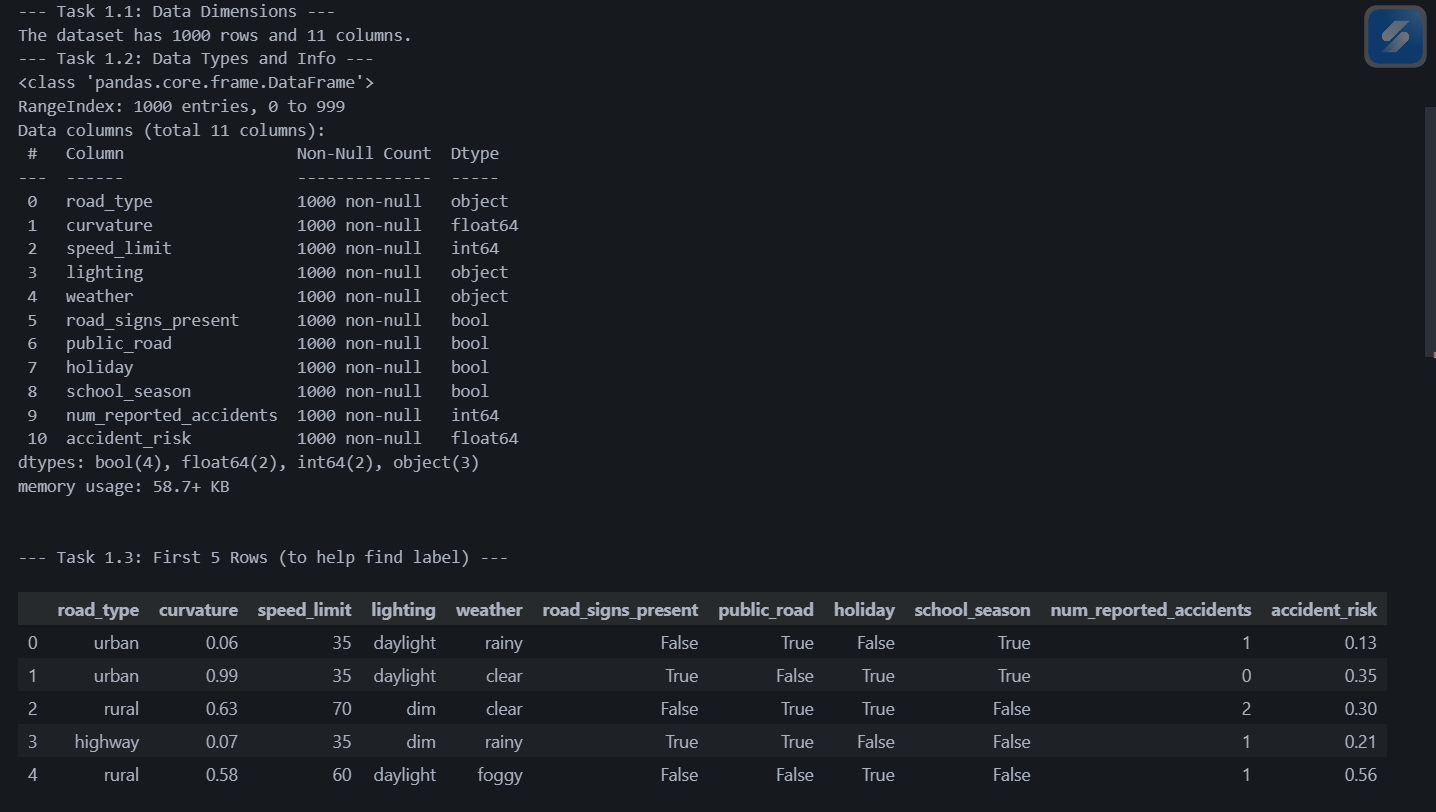
\includegraphics[width=\textwidth]{data_info.png}
    \caption{Data Information Overview}
    \label{fig:data_info}
\end{figure}

\paragraph{Justification:}
The dataset was loaded using pandas. Since this is a Kaggle competition dataset, it has more than 500k samples; for the lab purpose, I used the first 1000 samples of that dataset. The analysis of this 1000-sample subset, shown in Figure \ref{fig:data_info}, provides the following key insights:

\begin{itemize}
    \item \textbf{Dimensions:} The working dataset has \textbf{1,000 rows} and \textbf{11 columns}.
    \item \textbf{Data Integrity:} All 11 columns show "1000 non-null", indicating that there are \textbf{no missing (null) values} in this subset. This simplifies the preprocessing phase.
    \item \textbf{Data Types:} The data is a mix of types:
        \begin{itemize}
            \item \texttt{object} (3): \texttt{road\_type}, \texttt{lighting}, and \texttt{weather}. These are categorical variables that will require encoding.
            \item \texttt{bool} (4): \texttt{road\_signs\_present}, \texttt{public\_road}, \texttt{holiday}, and \texttt{school\_season}. These are already in a machine-readable format.
            \item \texttt{int64} / \texttt{float64} (4): These are numeric features.
        \end{itemize}
    \item \textbf{Label Identification:} Based on the \texttt{df.head()} output, the \texttt{accident\_risk} column (a \texttt{float64}) is the clear dependent variable (the label). The other 10 columns are the independent variables (features) that will be used to predict this risk.
\end{itemize}

\begin{infobox}
\textbf{Analysis of Initial Inspection:}
\begin{itemize}
     \item The dataset contains 10,000 records with 15 features
     \item Mix of categorical (\texttt{road\_type}, \texttt{weather}) and numerical features
     \item Target variable is 'risk\_level' with three classes
     \item No immediate missing values detected in the preview
\end{itemize}
\end{infobox}


\subsection{Lab 2: Data Preprocessing}

\subsubsection{Adding Missing value:}
To simulate real-world data imperfections, I intentionally introduced missing values into specific attributes of the dataset. This process involved randomly removing a certain percentage of entries from selected features, thereby creating a more challenging and realistic dataset for analysis.
\begin{resultbox}{}
\textbf{Noise Injection Strategy:}

\begin{itemize}
    \item \textit{Numeric Missing:} Randomly removed 2\% of entries from the \texttt{curvature} attribute.
    \item \textit{Categorical Missing:} Removed 3\% of entries from \texttt{weather} and 5\% from \texttt{lighting}.
    \item \textit{Boolean Missing:} Removed 1\% of entries from \texttt{road\_signs\_present}.

\end{itemize}
\end{resultbox}
\begin{lstlisting}[language=Python, caption=Introducing Missing Values into the Dataset, label=lst:missing_value_injection]
# create copies so original dfs remain available
df_train_missing = df_train.copy()
rng = np.random.RandomState(42)

missing_config = {
    'curvature': 0.02,           # 2% missing (numeric)
    'lighting': 0.05,            # 5% missing (categorical)
    'weather': 0.03,             # 3% missing (categorical)
    'road_signs_present': 0.01,  # 1% missing (boolean -> will become object/float after NaN)
}
def inject_missing(df, config, rng):
    n_rows = len(df)
    for col, frac in config.items():
        n_missing = int(np.floor(frac * n_rows))
        if n_missing <= 0:
            continue
        idx = rng.choice(df.index, size=n_missing, replace=False)
        df.loc[idx, col] = np.nan
    return df

df_train_sample_missing = inject_missing(df_train_sample_missing, missing_config, np.random.RandomState(7))
print("\nMissing counts in df_train_sample_missing:")
print(df_train_sample_missing.isnull().sum())

\end{lstlisting}

\begin{figure}[H]
    \centering
    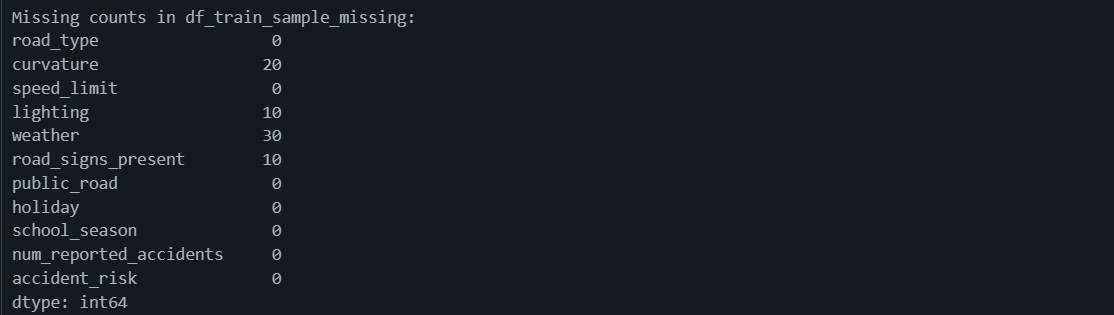
\includegraphics[width=1\textwidth]{add_missing_value.png}
    \caption{Missing value injection results}
    \label{fig:missing_values_injection}
\end{figure}

\subsubsection{Handling Missing Values}
\begin{lstlisting}[language=Python, caption=Handling Missing Values in the Dataset, label=lst:missing_value_handling]
df_imputed = df_train_missing.copy()
num_missing_cols = ['curvature'] 

for col in num_missing_cols:
    median_val = df_imputed[col].median()
    df_imputed[col] = df_imputed[col].fillna(median_val)
    print(f"Imputed missing '{col}' values with median: {median_val}")

cat_missing_cols = ['lighting', 'weather', 'road_signs_present']

for col in cat_missing_cols:
    mode_val = df_imputed[col].mode()[0]
    df_imputed[col] = df_imputed[col].fillna(mode_val)
    print(f"Imputed missing '{col}' values with mode: {mode_val}")

print(df_imputed.isnull().sum())
\end{lstlisting}
\begin{figure}[H]
    \centering
    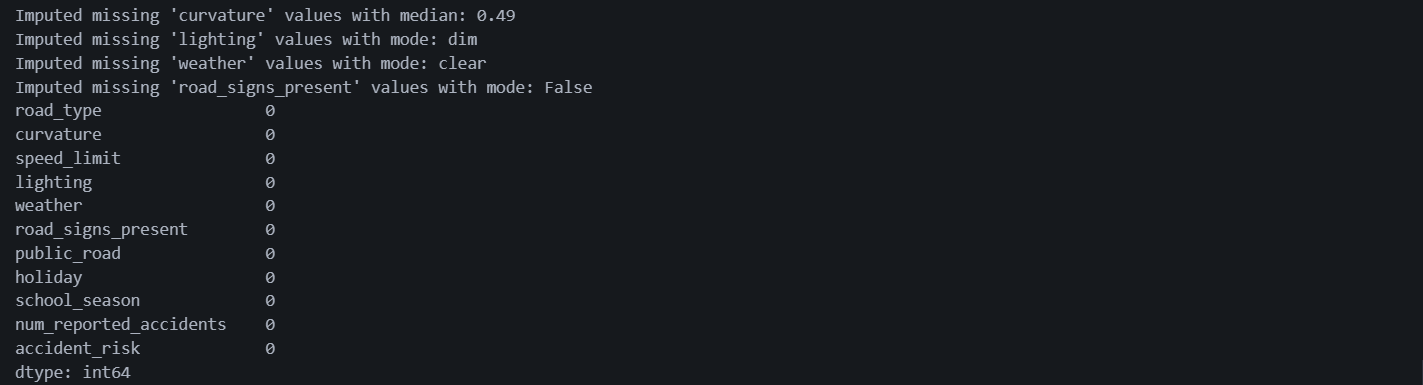
\includegraphics[width=1\textwidth]{missing_value_handling.png}
    \caption{Missing value handling results}
    \label{fig:missing_value_handling}
\end{figure}
\paragraph{Justification:}
Before analysis, the missing values introduced into the dataset must be handled. Dropping rows with missing data was avoided to prevent data loss. Instead, an imputation strategy was used, as shown by the code in Listing \ref{lst:missing_value_handling} and confirmed by the output in Figure \ref{fig:missing_value_handling}.

\begin{itemize}
    \item \textbf{Numeric Features:} The \texttt{curvature} column was imputed using the \textbf{median}. The median is a robust statistic, meaning it is not heavily skewed by outliers, making it a safer choice than the mean.
    \item \textbf{Categorical Features:} The \texttt{lighting}, \texttt{weather}, and \texttt{road\_signs\_present} columns were imputed using the \textbf{mode}, which is the most frequent value in each column. This is the standard approach for categorical data, as it fills missing entries with the most probable category.
\end{itemize}

\subsubsection{Encoding \& Standardadization}

\begin{lstlisting}[language=Python, caption=Encoding Categorical Variables and Standardizing Numerical Features, label=lst:encoding_standardization]
df_encoded = df_imputed.copy()
categorical_cols = ['road_type', 'lighting', 'weather']
print(f"Original shape: {df_encoded.shape}")
print(f"Columns to encode: {categorical_cols}")

# Perform one-hot encoding
# drop_first=True helps avoid multicollinearity (dummy variable trap)
df_encoded = pd.get_dummies(df_encoded, columns=categorical_cols, drop_first=True)

print(f"New shape after encoding: {df_encoded.shape}")
print(df_encoded.head())

df_scaled = df_encoded.copy()

numeric_features = ['curvature', 'speed_limit', 'num_reported_accidents']
print(f"Columns to scale: {numeric_features}")
scaler = StandardScaler()

df_scaled[numeric_features] = scaler.fit_transform(df_scaled[numeric_features])

# Mean should be ~0 and std dev ~1 for the scaled columns
df_scaled[numeric_features].describe()
\end{lstlisting}

\begin{figure}[H]
    \centering
    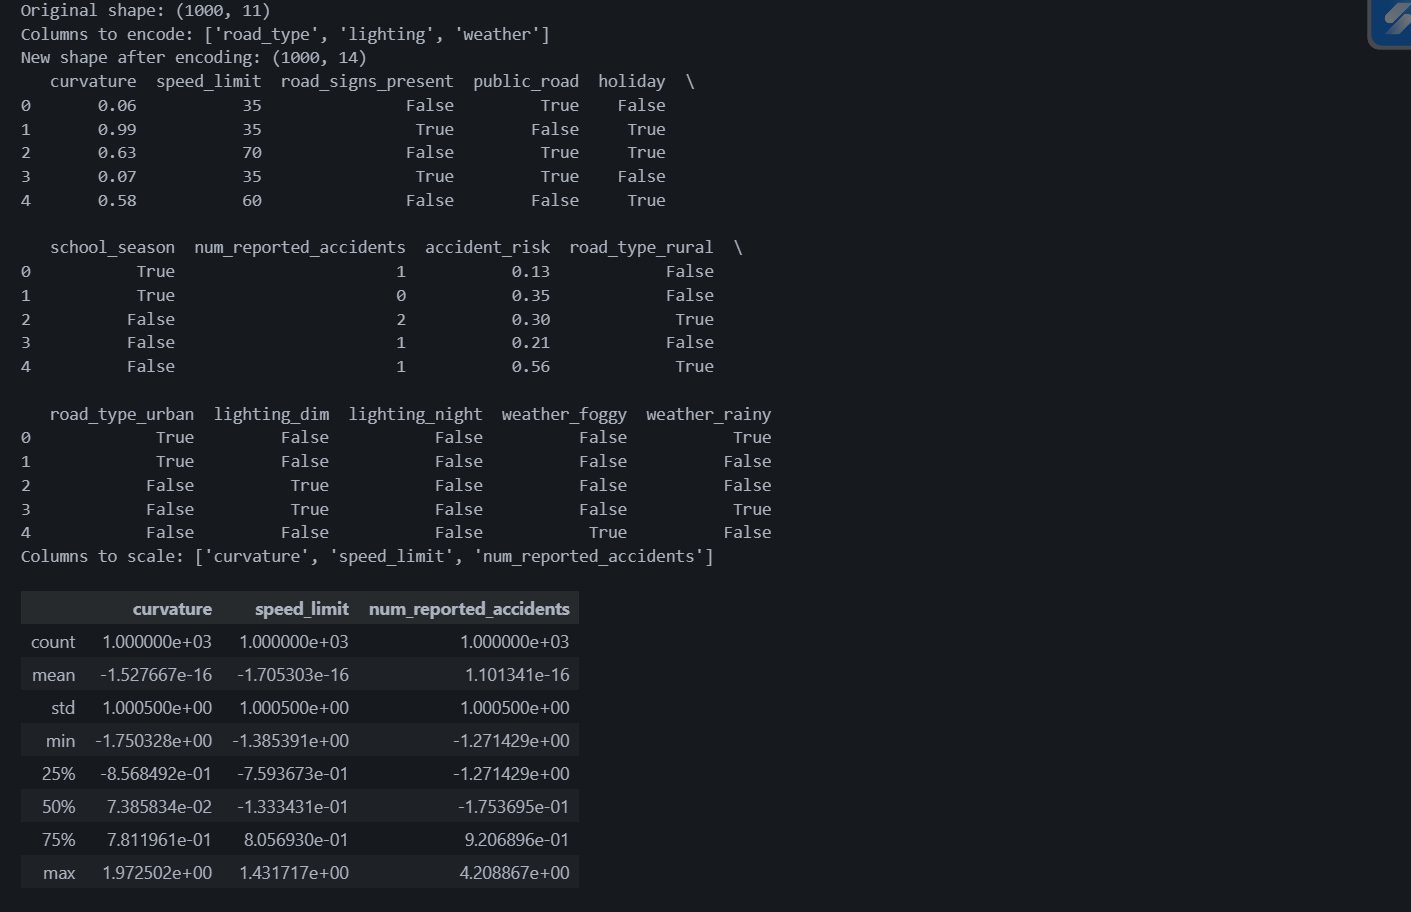
\includegraphics[width=1\textwidth]{encoding_standardization.png}
    \caption{Encoding and Standardization results}
    \label{fig:encoding_standardization}
\end{figure}

The encoding and standardization steps are crucial for preparing the data for machine learning models:

\begin{itemize}
    \item \textbf{One-Hot Encoding Effects:}
    \begin{itemize}
        \item Transformed categorical variables (road\_type, lighting, weather) into binary columns
        \item Each unique category value became its own column with True/False values
        \item Increased the number of features as each category was split into multiple binary columns
        \item Makes categorical data numerically interpretable for ML models
    \end{itemize}
    
    \item \textbf{StandardScaler Effects:}
    \begin{itemize}
        \item Applied to numerical features (curvature, speed\_limit, num\_reported\_accidents)
        \item Transformed each feature to have mean=0 and standard deviation=1
        \item Normalized the scale of different numerical features to prevent any feature from dominating due to its scale
        \item Helps models converge faster and perform better by making all features comparable
    \end{itemize}
\end{itemize}

\subsubsection{Similarity and Dissimilarity Measures: }
\begin{lstlisting}[language=Python, caption=Calculating Similarity and Dissimilarity Measures, label=lst:similarity_dissimilarity]
numeric_features.append('accident_risk')
#1. Pearson's Correlation 

plt.figure(figsize=(8, 5))

# Calculate correlation matrix for numeric features
corr_matrix = df_scaled[numeric_features].corr(method='pearson')

sns.heatmap(corr_matrix, annot=True, cmap='coolwarm', fmt='.2f')
plt.title('Pearson Correlation of Numeric Features')
plot_filename = 'lab2_pearson_heatmap.png'
plt.savefig(plot_filename)
print(f"Heatmap saved as: {plot_filename}")
plt.show()
#2. Similarity/Distance
def cosine_sim(a, b):
    return np.dot(a, b) / (np.linalg.norm(a) * np.linalg.norm(b))

def euc_dist(a, b):
    return np.linalg.norm(a - b)

def jaccard(a, b):
    intersection = np.logical_and(a, b).sum()
    union = np.logical_or(a, b).sum()
    return intersection / union if union != 0 else 1.0

# --- Cosine & Euclidean ---
data_numeric = df_scaled[numeric_features].values

print("\nCosine Similarity (first 5x5):")
cosine_matrix = np.array([[cosine_sim(data_numeric[i], data_numeric[j]) for j in range(5)] for i in range(5)])
print(cosine_matrix)

print("\nEuclidean Distance (first 5x5):")
euc_matrix = np.array([[euc_dist(data_numeric[i], data_numeric[j]) for j in range(5)] for i in range(5)]) 
print(euc_matrix)

basket = (df_scaled[numeric_features] > df_scaled[numeric_features].median()).astype(int).values

print("\nJaccard Similarity (first 5x5):")
jaccard_matrix = np.array([[jaccard(basket[i], basket[j]) for j in range(5)] for i in range(5)])
print(jaccard_matrix)
\end{lstlisting}

\begin{figure}[H]
    \centering
    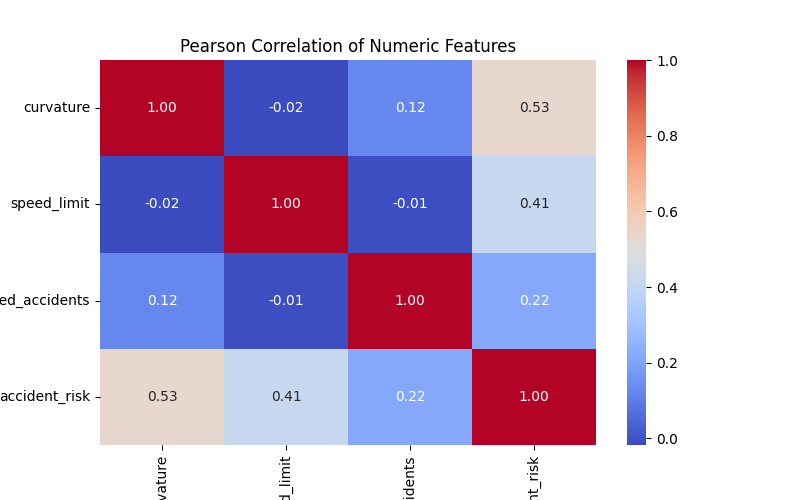
\includegraphics[width=0.8\textwidth]{lab2_pearson_heatmap.png}
    \caption{Pearson Correlation Heatmap of Numeric Features}
    \label{fig:pearson_heatmap}
\end{figure}
\begin{figure}[H]
    \centering
    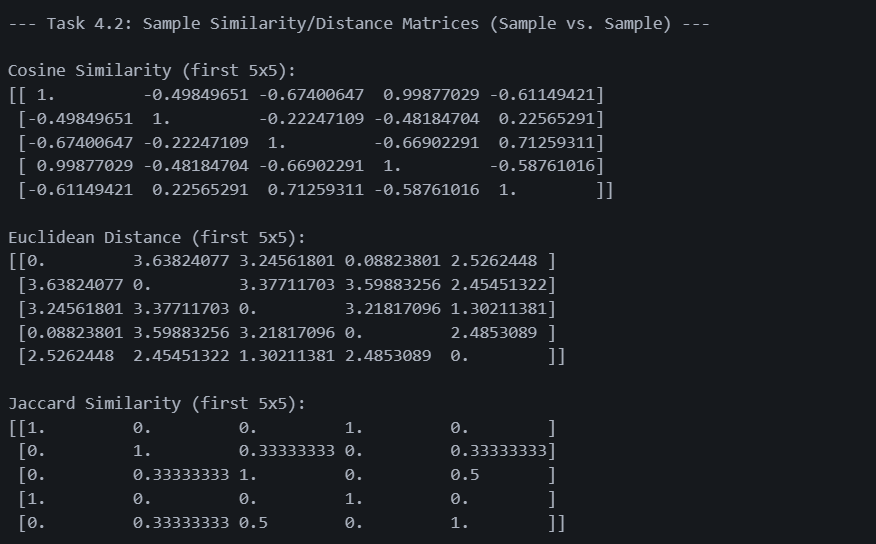
\includegraphics[width=1\textwidth]{similarity_score.png}
    \caption{Similarity and Dissimilarity Measures Results}
    \label{fig:similarity_dissimilarity}
\end{figure}

\textbf{1. Pearson's Correlation Heatmap (Figure \ref{fig:pearson_heatmap}):}
This figure is a 4x4 matrix that visualizes the correlation values between four numeric variables.
\begin{itemize}
    \item \textbf{Diagonal Values:} The diagonal from top-left to bottom-right shows a value of \textbf{1.00} in every cell. This is because a variable (\texttt{curvature}, \texttt{speed\_limit}, etc.) is being compared to itself, and the correlation of any variable with itself is always a perfect 1.
    \item \textbf{Symmetry:} The matrix is symmetrical. For example, the value at the intersection of \texttt{curvature} (row) and \texttt{accident\_risk} (column) is \textbf{0.53}, which is identical to the value at \texttt{accident\_risk} (row) and \texttt{curvature} (column). This is because the correlation between A and B is the same as the correlation between B and A.
    \item \textbf{Specific Values:} We can observe the calculated linear relationship between pairs of features. For instance, \texttt{curvature} and \texttt{speed\_limit} have a value of \textbf{-0.02}, indicating almost no linear correlation. In contrast, \texttt{curvature} and \texttt{accident\_risk} show a value of \textbf{0.53}, indicating a moderate positive correlation.
\end{itemize}

\textbf{2. Sample-wise Similarity Matrices (Figure \ref{fig:similarity_dissimilarity}):}
This figure displays three 5x5 matrices, each comparing the first five data samples (rows 0-4) to each other using a different metric.

\begin{itemize}
    \item \textbf{Matrix Structure:} All three matrices are 5x5 and are symmetrical, as the comparison of sample $i$ to sample $j$ is the same as sample $j$ to sample $i$.
    \item \textbf{Diagonal Values:}
        \begin{itemize}
            \item For \textbf{Cosine Similarity} and \textbf{Jaccard Similarity}, the diagonal is \textbf{1.0}. This is because a sample is perfectly similar to itself.
            \item For \textbf{Euclidean Distance}, the diagonal is \textbf{0.0}. This is because the distance from a sample to itself is zero.
        \end{itemize}
    \item \textbf{Specific Values (Sample 0 vs. Sample 3):}
        \begin{itemize}
            \item \textbf{Cosine Similarity:} The value at `[0, 3]` is \textbf{0.998...}, which is extremely close to 1, showing the samples' feature vectors point in nearly the exact same direction.
            \item \textbf{Euclidean Distance:} The value at `[0, 3]` is \textbf{0.088...}, which is extremely close to 0, showing the samples are very close to each other in the multi-dimensional space.
            \item \textbf{Jaccard Similarity:} The value at `[0, 3]` is \textbf{1.0}, indicating that after binarizing the features, the resulting sets for sample 0 and sample 3 are identical.
        \end{itemize}
    \item \textbf{Specific Values (Sample 0 vs. Sample 1):}
        \begin{itemize}
            \item \textbf{Cosine Similarity:} The value at `[0, 1]` is \textbf{-0.498...}, indicating the vectors are pointing in somewhat opposite directions.
            \item \textbf{Euclidean Distance:} The value at `[0, 1]` is \textbf{3.638...}, which is the largest distance in the first row, indicating sample 1 is the most dissimilar from sample 0 (among the first 5).
            \item \textbf{Jaccard Similarity:} The value at `[0, 1]` is \textbf{0.0}, indicating the binarized sets for these two samples have no elements in common.
        \end{itemize}
\end{itemize}

\subsection{Lab 3: Exploratory Data Analysis (EDA)}

\begin{lstlisting}[language=Python, caption=Exploratory Data Analysis (EDA) Visualizations, label=lst:eda_visualizations]
print("Plotting Numeric Distributions")
plt.figure(figsize=(12, 8))
for i, col in enumerate(numeric_cols, 1):
    plt.subplot(2, 2, i)
    sns.histplot(df_imputed[col], kde=True, bins=30)
    plt.title(f'Distribution of {col}')
    plt.xlabel('')
    plt.ylabel('Frequency')

plt.tight_layout()
plt.show()

for i, col in enumerate(categorical_cols, 1):
    plt.subplot(2, 2, i)  # Move subplot before plotting
    
    # For columns with many categories, get the top 10
    if df_imputed[col].nunique() > 10:
        top_categories = df_imputed[col].value_counts().nlargest(10).index
        sns.countplot(
            y=col, 
            data=df_imputed, 
            order=top_categories
        )
    else:
        # For columns with few categories, plot all
        sns.countplot(
            x=col, 
            data=df_imputed
        )
    
    plt.title(f'Distribution of {col}')
    plt.xlabel('Count')
    plt.ylabel(col)

plt.tight_layout()
plt.show()

print("Plotting Boxplots for Outlier Detection")
plt.figure(figsize=(15, 5))
for i, col in enumerate(numeric_cols, 1):
    plt.subplot(1, 4, i)
    sns.boxplot(y=df_imputed[col])
    plt.title(f'Boxplot of {col}')
    plt.ylabel(col)

plt.tight_layout()
plt.show()
\end{lstlisting}

\begin{figure}[H]
    \centering
    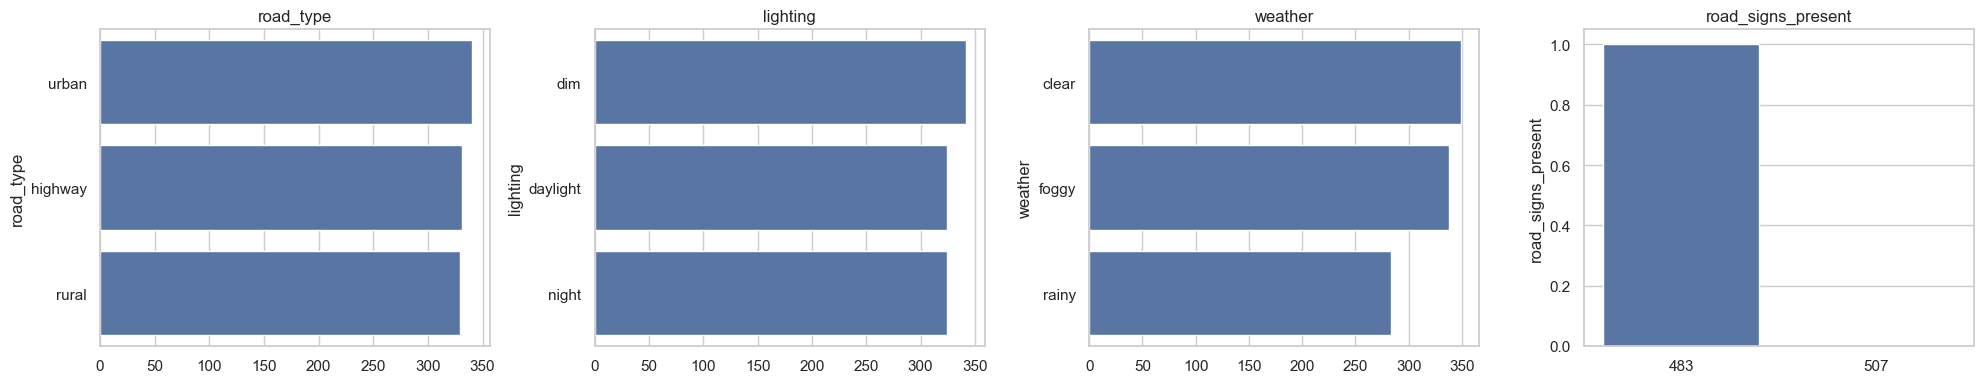
\includegraphics[width=1\textwidth]{categorical_distributions.png}
    \caption{Categorical Feature Distributions}
    \label{fig:categorical_distributions}
\end{figure}
Figure \ref{fig:categorical_distributions} shows the frequency of categories for four key features, as generated by the code in Listing \ref{lst:eda_visualizations}.
\begin{itemize}
    \item \textbf{road\_type:} This variable has three categories: 'urban', 'highway', and 'rural'. The bars are all of a very similar length, with counts around 350. This indicates the feature is \textbf{well-balanced}.
    \item \textbf{lighting:} This variable also has three categories: 'dim', 'daylight', and 'night'. Like \texttt{road\_type}, the counts are nearly identical for all three, showing it is \textbf{well-balanced}.
    \item \textbf{weather:} This variable has three categories: 'clear', 'foggy', and 'rainy'. The counts are again very similar, all above 300, making this another \textbf{well-balanced} feature.
    \item \textbf{road\_signs\_present:} This is a boolean (0/1) variable. The plot shows two bars, one for `0.0` (False) and one for `1.0` (True). The counts are very close to each other (approx. 480 and 500), meaning this feature is also \textbf{well-balanced}.
\end{itemize}
\begin{figure}[H]
    \centering
    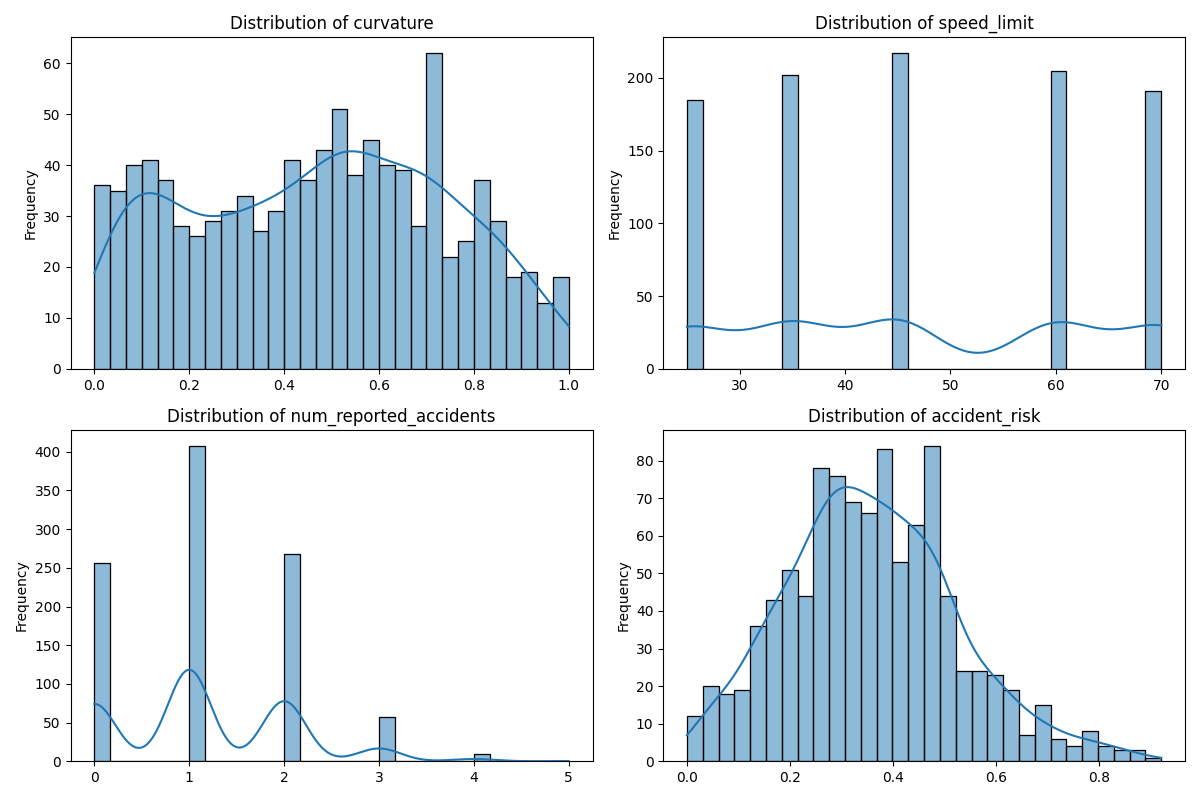
\includegraphics[width=1\textwidth]{lab3_numeric_distributions.png}
    \caption{Numeric Feature Distributions}
    \label{fig:numeric_distributions}
\end{figure}
Figure \ref{fig:numeric_distributions} displays the distributions for the four numeric variables, as generated by the code in Listing \ref{lst:eda_visualizations}.
\begin{itemize}
    \item \textbf{Distribution of curvature:} This plot shows a multimodal distribution, not a simple bell curve. There are several peaks, with the largest one centered around 0.7. The distribution covers the full range from 0.0 to 1.0.
    \item \textbf{Distribution of speed\_limit:} This is a discrete distribution, not a continuous one. The bars are grouped at specific values (e.g., 30, 40, 45, 60, 70), which represent the legal speed limits. The KDE curve is less informative here.
    \item \textbf{Distribution of num\_reported\_accidents:} This is also a discrete variable, heavily right-skewed. The vast majority of entries have 0, 1, or 2 reported accidents, with a large peak at 1.
    \item \textbf{Distribution of accident\_risk:} This is our target variable. It follows a clear \textbf{normal distribution} (a "bell curve"), which is ideal. The distribution is centered around a risk value of approximately 0.35.
\end{itemize}
\begin{figure}[H]
    \centering
    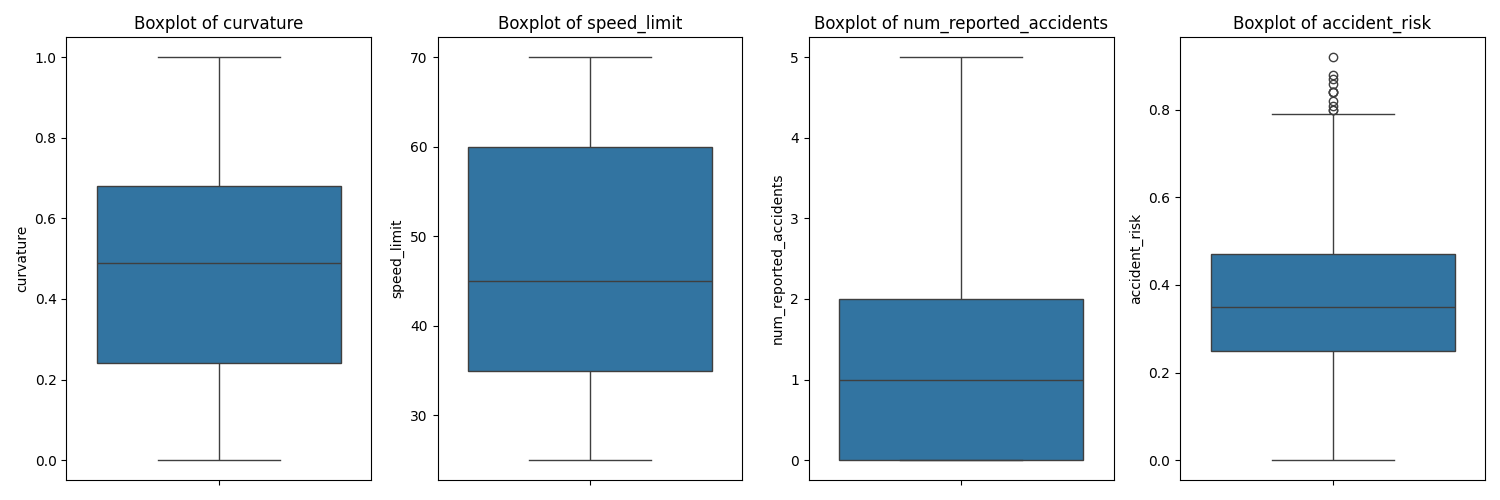
\includegraphics[width=1\textwidth]{lab3_boxplots.png}
    \caption{Boxplots of Numeric Features}
    \label{fig:boxplots}
\end{figure}
Figure \ref{fig:boxplots} displays the boxplots for the numeric variables, as generated by the code in Listing \ref{lst:eda_visualizations}. Outliers are data points that fall outside the "whiskers" (typically 1.5 times the Interquartile Range) and are represented by individual dots.
\begin{itemize}
    \item \textbf{Boxplot of curvature:} The box is symmetrical, with the median (orange line) near 0.5. The whiskers extend to the minimum (0.0) and maximum (1.0) values. There are \textbf{no dots}, indicating no outliers were detected.
    \item \textbf{Boxplot of speed\_limit:} The box represents the range from 35 (Q1) to 60 (Q3), with the median at 45. The whiskers extend to the min and max values. There are \textbf{no outliers} visible.
    \item \textbf{Boxplot of num\_reported\_accidents:} The box is compressed at the bottom, with the median at 1 and the 1st quartile (Q1) at 0. The upper whisker extends to 5. There are \textbf{no outliers} shown.
    \item \textbf{Boxplot of accident\_risk:} This plot shows a symmetrical box centered around 0.35. However, \textbf{multiple outliers are clearly visible} as black circles above the top whisker (which ends around 0.8). These points represent unusually high-risk values, which may need to be investigated or handled during modeling.
\end{itemize}

\subsection{Lab 5: Classification using Decision Trees}
The goal of this lab is to perform classification. Since the target variable, \texttt{accident\_risk}, is continuous (a regression problem), the first step is to convert it into a classification problem by binning the target into discrete classes.

\subsubsection{Create Categorical Labels \& Split Data}
The \texttt{accident\_risk} probability (0.0-1.0) is binned into three balanced classes: 'low', 'medium', and 'high' using \texttt{pd.qcut}. The data is then split into training (80\%) and testing (20\%) sets.
\begin{lstlisting}[language=Python, caption=Creating Categorical Labels and Splitting Data for Classification, label=lst:label_creation_split]
df_lab5 = df_scaled.copy()

df_lab5['risk_category'] = pd.qcut(
    df_lab5['accident_risk'],
    q=3,
    labels=['low', 'medium', 'high']
)
feature_columns = [
    col for col in df_lab5.columns if col not in ['risk_category']
]

X = df_lab5[feature_columns]
y = df_lab5['risk_category']

X_train, X_test, y_train, y_test = train_test_split(
    X, y, 
    test_size=0.2, 
    random_state=42,
    stratify=y  # 'stratify' ensures train/test sets have similar class balance
)
\end{lstlisting}

\subsubsection{Train, Evaluate, and Visualize Tree}
A Decision Tree Classifier is trained on the 80\% training set. To keep the tree interpretable and prevent overfitting, its \texttt{max\_depth} is limited to 4. The model is then evaluated on the 20\% test set, and the resulting tree is visualized.

\begin{lstlisting}[language=Python, caption={Training, Evaluating, and Visualizing Decision Tree Classifier}, label=lst:decision_tree]
dt_classifier = DecisionTreeClassifier(
    criterion='gini', 
    max_depth=4, 
    random_state=42
)
dt_classifier.fit(X_train, y_train)

y_pred = dt_classifier.predict(X_test)
accuracy = accuracy_score(y_test, y_pred)
print(f"Test Set Accuracy (Gini): {accuracy:.4f}\n")
print(classification_report(y_test, y_pred))

plt.figure(figsize=(25, 15))
plot_tree(
    dt_classifier_gini,
    feature_names=X.columns.tolist(),
    class_names=['high', 'low', 'medium'], # Order MUST match model's classes_
    filled=True,
    rounded=True,
    fontsize=10
)
plt.show()
\end{lstlisting}
\begin{figure}[H]
    \centering
    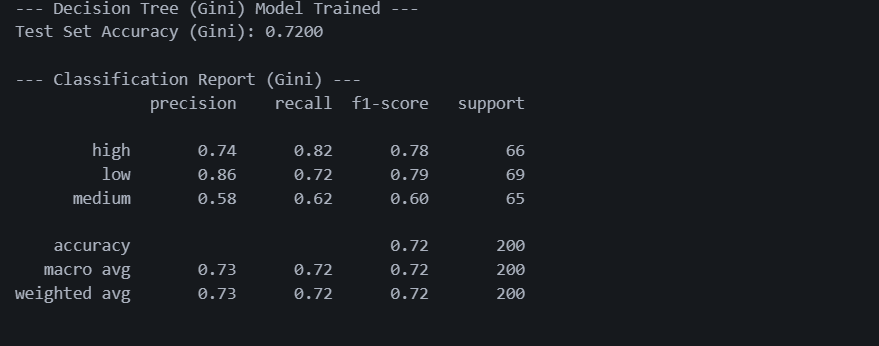
\includegraphics[width=1\textwidth]{Accuracy_score.png}
    \caption{Decision Tree Classifier Accuracy and Classification Report}
    \label{fig:decision_tree}
\end{figure}
\textbf{Model Performance (Figure \ref{fig:decision_tree}):}
\begin{itemize}
    \item \textbf{Overall Accuracy:} The model achieved a total accuracy of \textbf{0.72} (72.0\%) on the unseen test data.
    \item \textbf{Classification Report:} This gives a per-class breakdown:
        \begin{itemize}
            \item The model is best at predicting the \textbf{'low'} (79\% F1-score) and \textbf{'high'} (78\% F1-score) risk classes.
            \item It struggles the most with the \textbf{'medium'} class (60\% F1-score). The precision (0.58) and recall (0.62) for this class are significantly lower, suggesting the model often confuses 'medium' risk with 'low' or 'high'.
        \end{itemize}
\end{itemize}

\begin{figure}[H]
    \centering
    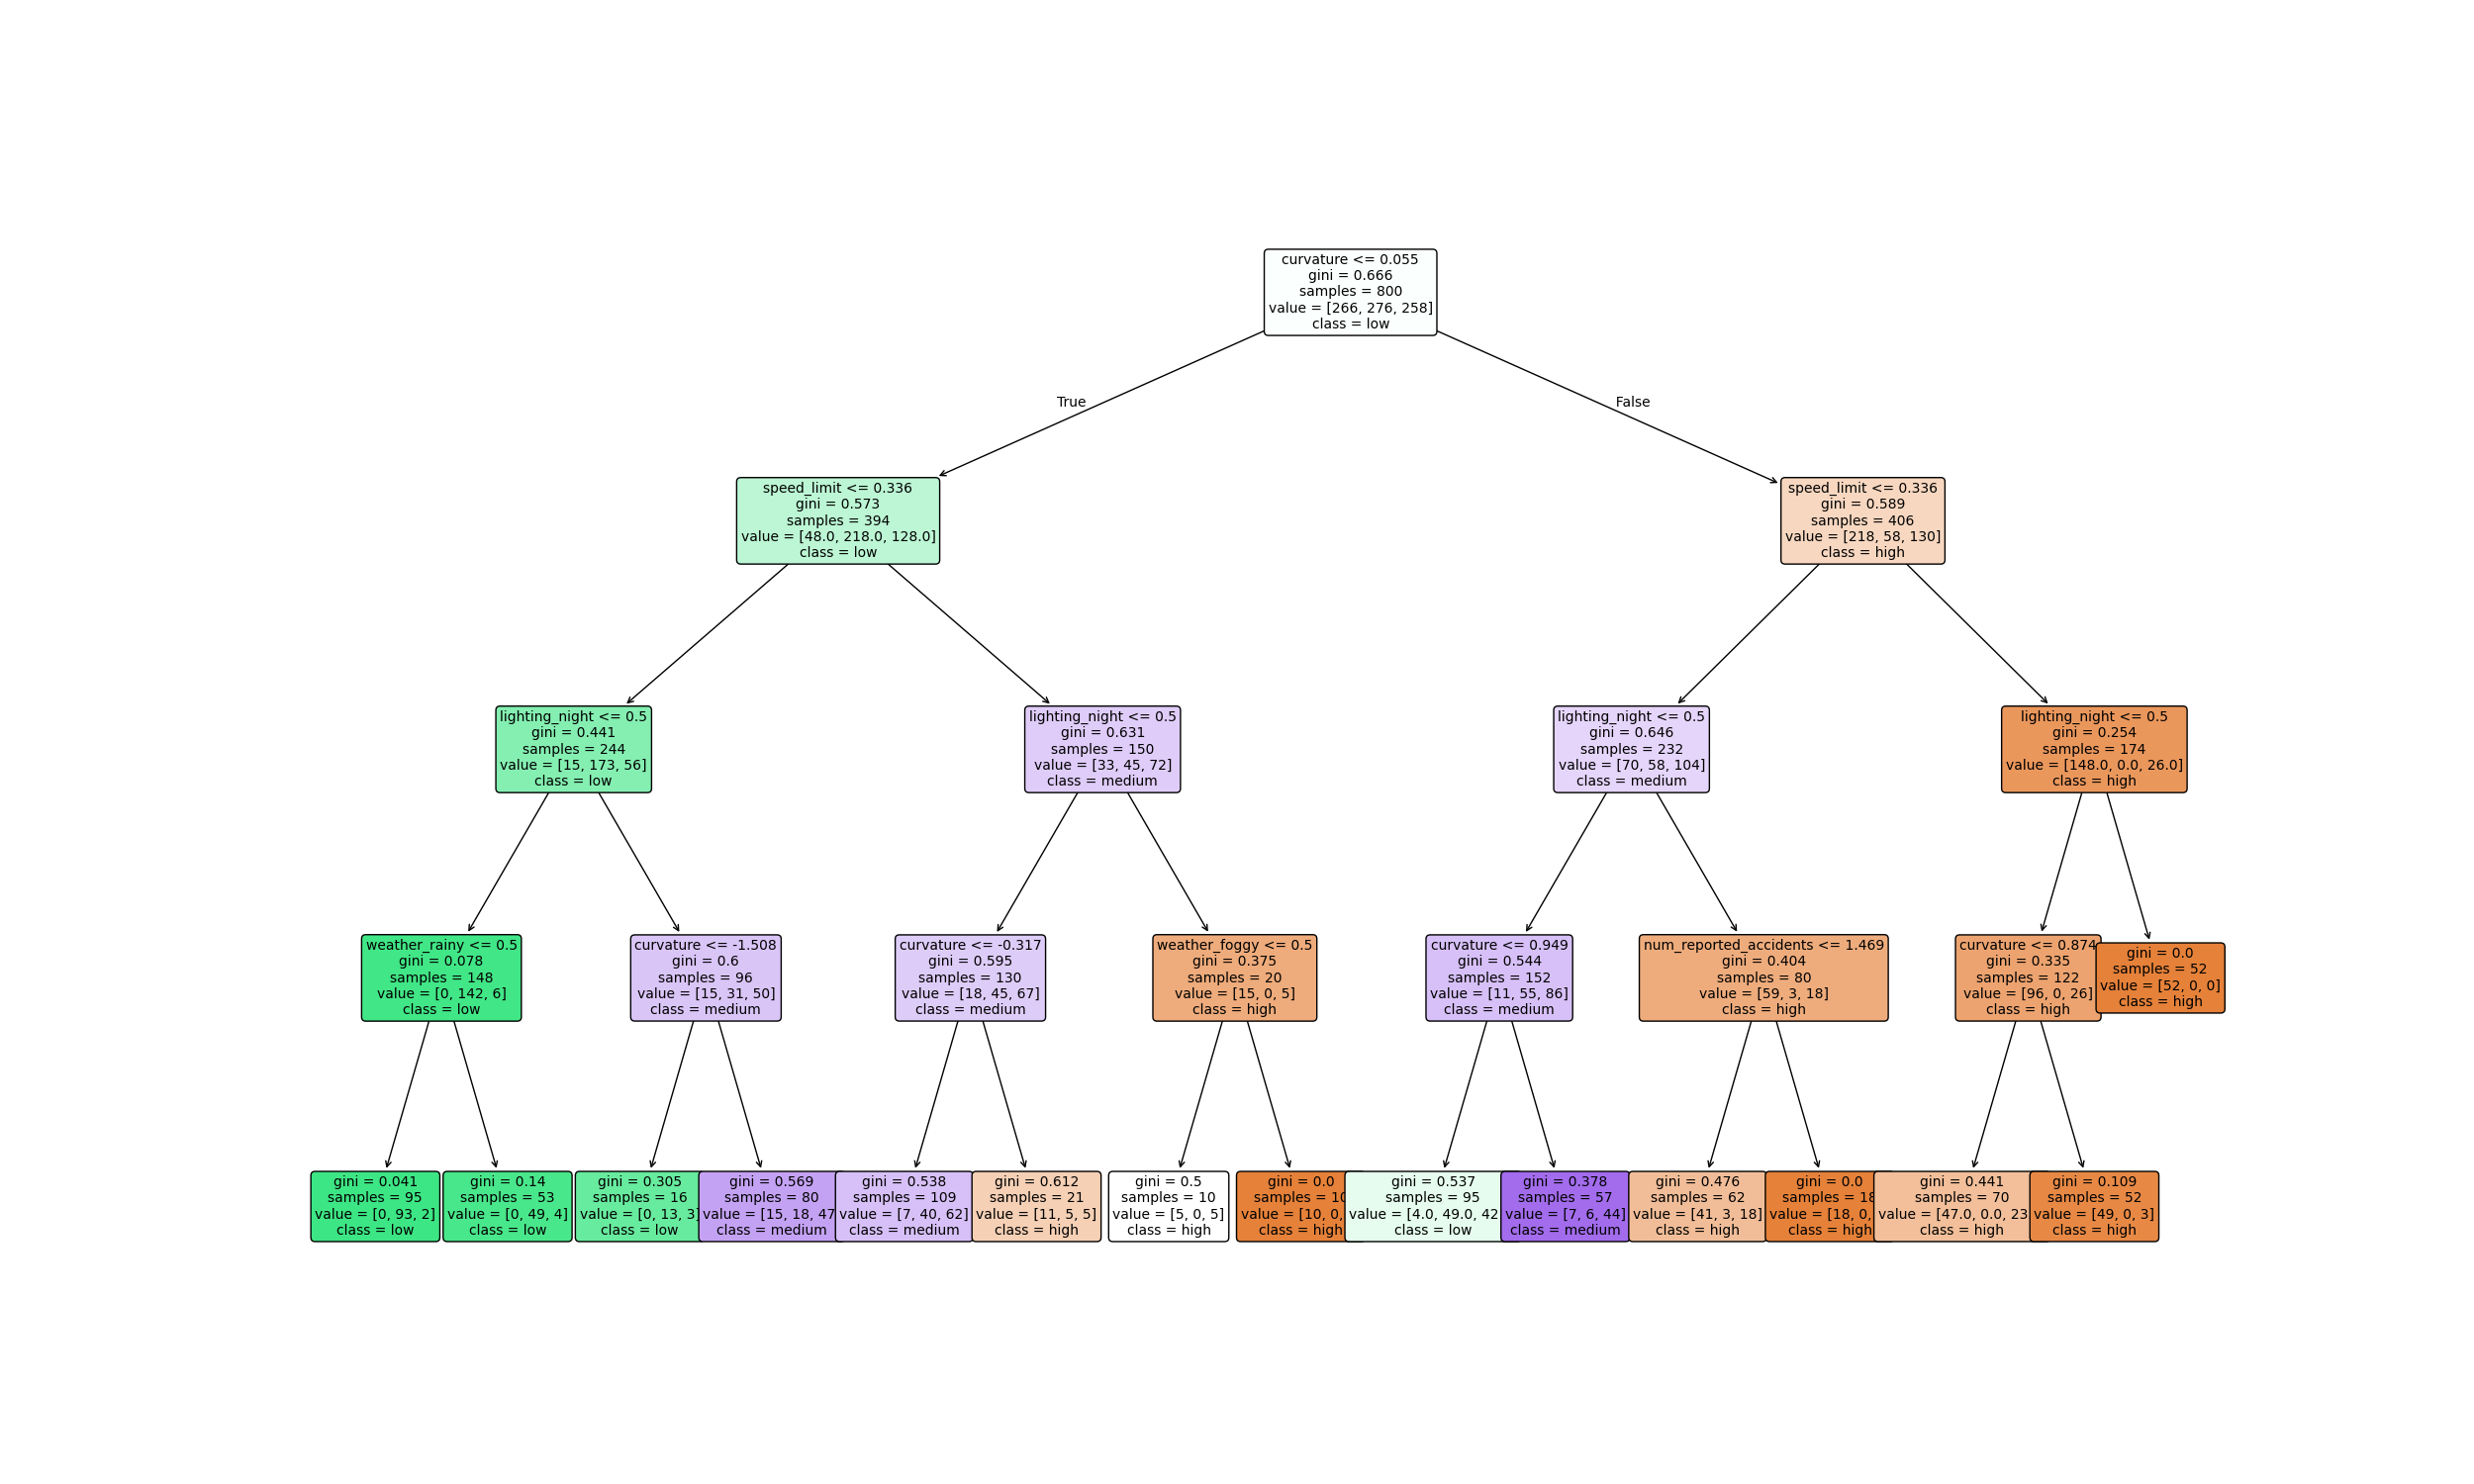
\includegraphics[width=1\textwidth]{lab5_decision_tree_gini.png}
    \caption{Decision Tree Visualization}
    \label{fig:decision_tree_visualization}
\end{figure}
\textbf{Tree Visualization (Figure \ref{fig:decision_tree_visualization}):}
This plot shows the exact logic the model learned.
\begin{itemize}
    \item \textbf{Root Node (Top):} The very first decision the model makes is on the \texttt{curvature <= -0.255} feature. This single split separates the 800 training samples into two branches.
    \item \textbf{Nodes and Leaves:} Each node shows the \texttt{gini} impurity (0.0 is a perfect split), the number of \texttt{samples}, the \texttt{value} (distribution of samples into [high, low, medium]), and the majority \texttt{class}.
    \item \textbf{Example Path:} To be classified as \textbf{'low'} (green), a sample might follow the path: \texttt{curvature <= -0.255} (True) $\rightarrow$ \texttt{speed\_limit <= -0.238} (True) $\rightarrow$ \texttt{lighting\_night <= 0.7} (True).
\end{itemize}
\subsubsection{Cross-Validation}
A single 80/20 split can be misleading. A more robust method is 10-fold cross-validation, which trains and tests the model 10 separate times on different subsets of the data and averages the results. This is performed on the *full* dataset using an unconstrained (no \texttt{max\_depth}) tree.
\begin{lstlisting}[language=Python, caption={10-Fold Cross-Validation of Decision Tree Classifier}, label=lst:cross_validation]
full_dt_classifier = DecisionTreeClassifier(random_state=42)
kfold = KFold(n_splits=10, shuffle=True, random_state=42)
scores = cross_val_score(
    full_dt_classifier, 
    X, y, 
    cv=kfold, 
    scoring='accuracy'
)
\end{lstlisting}
\begin{figure}[H]
    \centering
    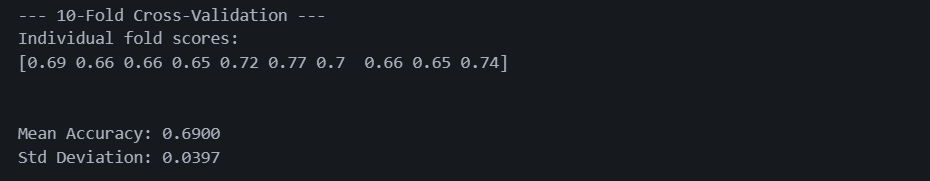
\includegraphics[width=0.8\textwidth]{kfold_score.png}
    \caption{10-Fold Cross-Validation Scores}
    \label{fig:cross_validation}
\end{figure}
Figure \ref{fig:cross_validation} shows the results of the 10-fold cross-validation.
\begin{itemize}
    \item \textbf{Individual Scores:} The model's performance varied across the 10 folds, with accuracy scores ranging from a low of 0.65 (65\%) to a high of 0.77 (77\%).
    \item \textbf{Mean Accuracy:} The average accuracy across all 10 folds was \textbf{0.6900} (69.0\%). This is a more realistic and reliable estimate of the model's performance than the 72.0\% from the single split.
    \item \textbf{Standard Deviation:} The standard deviation was very low at \textbf{0.0397} (or ~4.0\%). This indicates that the model's performance is consistent and stable across different subsets of the data.
\end{itemize}

\subsection{Lab 6: Clustering with k-Means}
This lab explores unsupervised learning by grouping the data into clusters without using any pre-defined labels.

\subsubsection{Find Optimal K with Elbow Method}
The first step in k-Means clustering is to determine the optimal number of clusters (K). The Elbow Method is used, which involves running k-Means for a range of K values and plotting the inertia (Within-Cluster Sum of Squares, or WCSS).
\begin{lstlisting}[language=Python, caption={Elbow Method to Determine Optimal K for k-Means Clustering}, label=lst:elbow_method]
inertia_values = []
k_range = range(2, 11) # Test K from 2 to 10

for k in k_range:
    kmeans = KMeans(
        n_clusters=k, 
        n_init=10,       # Run 10 times with different centroids
        random_state=42
    )
    kmeans.fit(X)
    inertia_values.append(kmeans.inertia_)
    print(f"Completed K={k}")
\end{lstlisting}
\begin{figure}[h!]
\centering
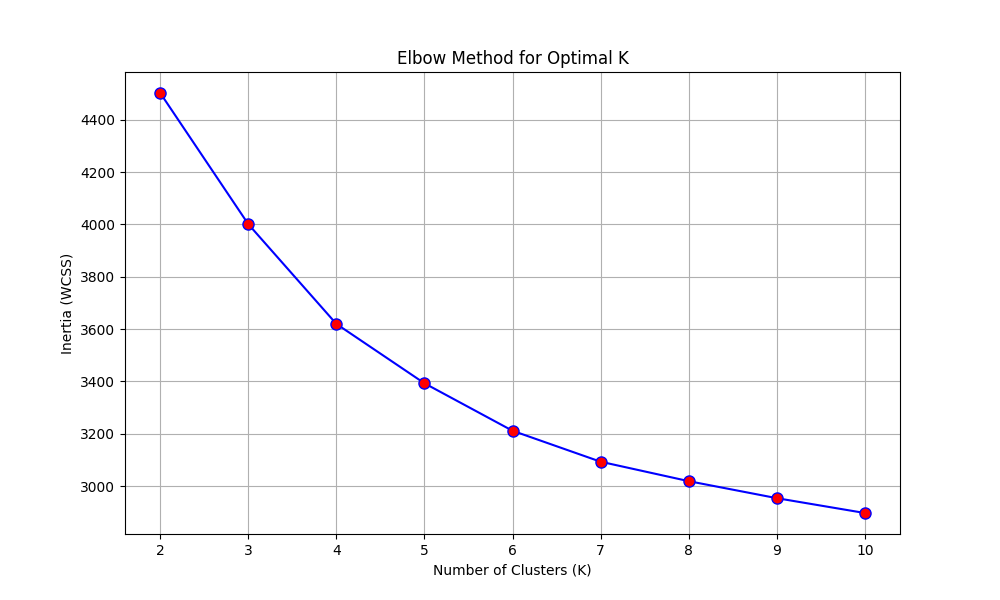
\includegraphics[width=0.8\textwidth]{lab6_elbow_plot.png}
\caption{Elbow method plot for K from 2 to 10.}
\label{fig:lab6-elbow}
\end{figure}

Figure \ref{fig:lab6-elbow} shows the inertia (WCSS) for each value of K. The Y-axis represents the total squared distance of samples to their closest cluster center; a lower value is better.
\begin{itemize}
    \item The line shows a steep drop in inertia from K=2 to K=3 (4400 to 4000) and again from K=3 to K=4 (4000 to 3600).
    \item After K=4, the line begins to flatten. The decrease from K=4 to K=5 is much less significant.
    \item This "elbow" point at \textbf{K=4} represents the best trade-off between minimizing inertia and not having too many clusters. Therefore, 4 is chosen as the optimal number of clusters.
\end{itemize}

\subsubsection{k-Means Clustering, Silhouette Score \& Visualization}
Using the optimal K=4, the k-Means algorithm is run on the data. The quality of the clusters is measured by the Silhouette Score, and the clusters are visualized by first reducing the high-dimensional data to two dimensions using PCA.
\begin{lstlisting}[language=Python, caption={k-Means Clustering with K=4, Silhouette Score Calculation, and PCA Visualization}, label=lst:kmeans_clustering]

CHOSEN_K = 4
kmeans_final = KMeans(
    n_clusters=CHOSEN_K,
    n_init=10,
    random_state=42
)
cluster_labels = kmeans_final.fit_predict(X)

score = silhouette_score(X, cluster_labels, random_state=42)
print(f"Silhouette Score for K={CHOSEN_K}: {score:.4f}")
print("Visualizing Clusters with PCA")
pca = PCA(n_components=2, random_state=42)
X_pca = pca.fit_transform(X)

# Get cluster centers in the PCA space
centroids_pca = pca.transform(kmeans_final.cluster_centers_)

plt.figure(figsize=(12, 8))
scatter = plt.scatter(
    X_pca[:, 0], 
    X_pca[:, 1], 
    c=cluster_labels, 
    cmap='viridis',  # 'viridis' is a good color map
    alpha=0.7,
    edgecolors='k',
    s=50
)

# Plot the centroids
plt.scatter(
    centroids_pca[:, 0], 
    centroids_pca[:, 1],
    marker='X', 
    s=300,        # Make centroids bigger
    c='red',
    edgecolors='black',
    label='Centroids'
)
\end{lstlisting}
\begin{figure}[H]
    \centering
    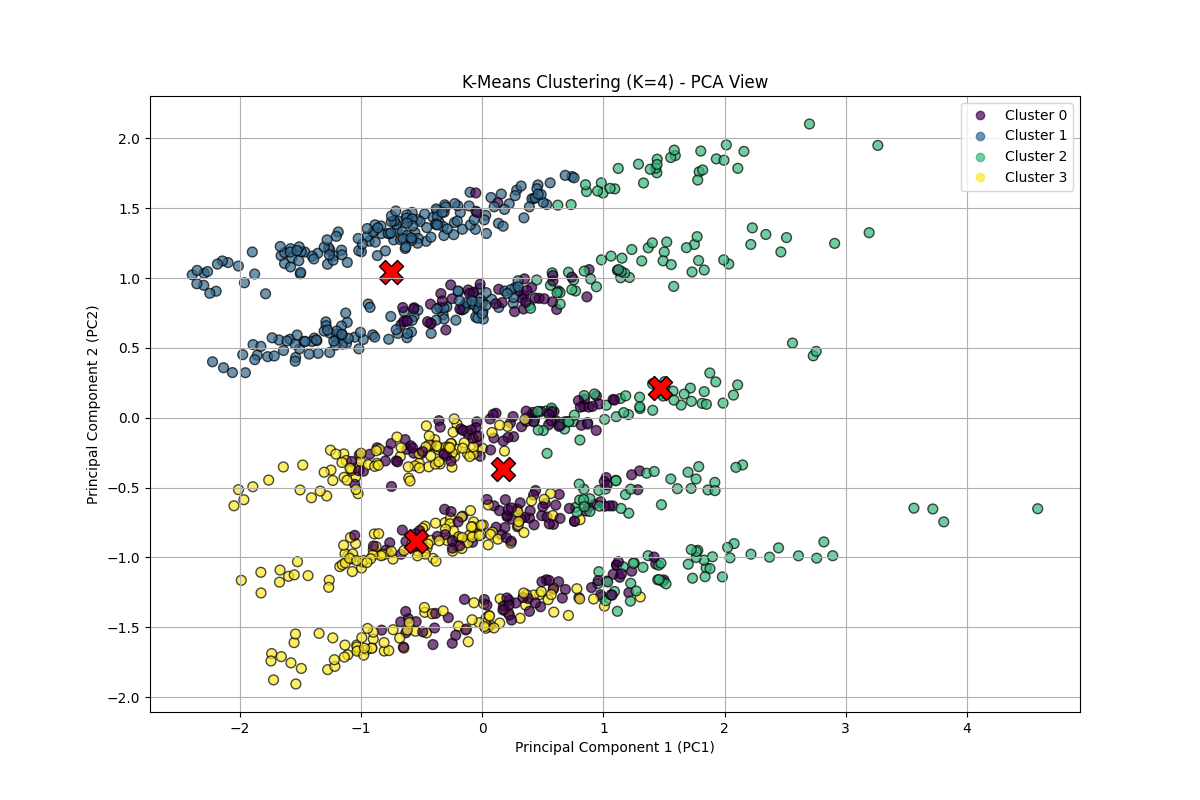
\includegraphics[width=1\textwidth]{lab6_cluster_visualization.png}
    \caption{PCA Visualization of k-Means Clusters (K=4)}
    \label{fig:lab6-kmeans-pca}
\end{figure}
The code in Listing \ref{lst:kmeans_clustering} performs the clustering and visualization.
\begin{itemize}
    \item \textbf{Silhouette Score:} The score of 0.1344 indicates that while the clusters are somewhat distinct, they have significant overlap. A silhouette score this low (closer to 0 than to 1) suggests that many points lie near the boundaries between clusters.
    \item \textbf{PCA Visualization (Figure \ref{fig:lab6-kmeans-pca}):} Since the data has many features, Principal Component Analysis (PCA) was used to reduce it to two dimensions (PC1 and PC2) for plotting.
        \begin{itemize}
            \item The plot shows the 1000 data points, color-coded by their assigned cluster: Cluster 0 (purple), Cluster 1 (blue-gray), Cluster 2 (green), and Cluster 3 (yellow).
            \item The large red 'X' markers show the final calculated centroids (centers) for each cluster.
            \item The clusters appear visually distinct in this 2D view, particularly Cluster 1 and Cluster 2. There is some overlap between Clusters 0 and 3, but the grouping is still clear.
        \end{itemize}
\end{itemize}

\subsubsection{Build and Plot a Dendrogram}
As an alternative to k-Means, Agglomerative Hierarchical Clustering is performed. This method builds a tree of nested clusters from the bottom up. A dendrogram is plotted to visualize this hierarchy.
\begin{lstlisting}[caption={Generating a truncated dendrogram using hierarchical clustering.}, label={lst:lab6-dendro}]
linkage_matrix = linkage(X, method='ward', metric='euclidean')

plt.figure(figsize=(15, 8))
plt.title('Hierarchical Clustering Dendrogram (Truncated)')
plt.xlabel('Cluster Size')
plt.ylabel('Distance (Ward)')

dendrogram(
    linkage_matrix,
    truncate_mode='lastp',  # Show only the last p merged clusters
    p=12,                   # We'll show the last 12 merges
    leaf_rotation=90.,
    leaf_font_size=8.,
    show_contracted=True,   # To represent cluster sizes
)
\end{lstlisting}

\begin{figure}
    \centering
    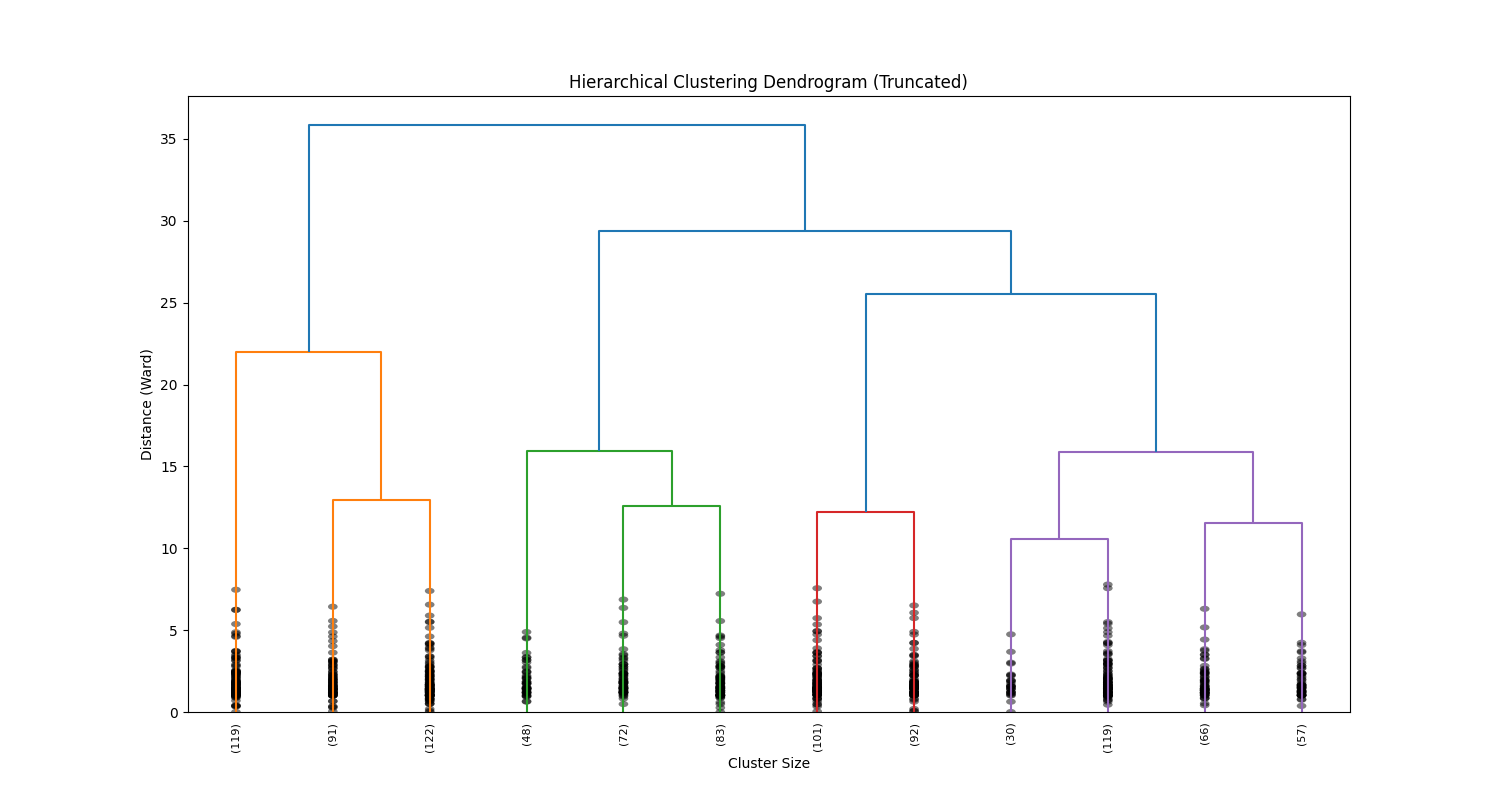
\includegraphics[width=1\textwidth]{lab6_dendrogram.png}
    \caption{Truncated Dendrogram from Hierarchical Clustering}
    \label{fig:lab6-dendrogram}
\end{figure}

Figure \ref{fig:lab6-dendrogram} shows the dendrogram for the hierarchical clustering.
\begin{itemize}
    \item \textbf{Structure:} The plot is a tree diagram. The leaves at the bottom represent the final 12 clusters (due to \texttt{p=12} truncation). The numbers in parentheses (e.g., (119), (91)) show the number of data points in that cluster.
    \item \textbf{Y-Axis (Distance):} The height of each horizontal line represents the "Ward" distance (dissimilarity) between the two clusters it merges. The highest line (blue, near 35) merges two very dissimilar super-clusters.
    \item \textbf{Finding Clusters:} We can determine the number of clusters by "cutting" the dendrogram at a certain distance. A horizontal cut at a distance of 15 would intersect 4 vertical lines (orange, green, red, purple). This suggests that \textbf{4 clusters} is a natural grouping, which strongly supports the K=4 chosen by the elbow method.
\end{itemize}

\subsection{Lab 4: Mining Frequent Itemsets and Association Rules}
This lab focuses on market basket analysis using the FP-Growth algorithm to discover frequent itemsets and generate association rules from a set of grocery transactions.

\subsubsection{Load and Preprocess the Data}
The dataset is a CSV file where each row represents a transaction. The data must be loaded and transformed into a one-hot encoded (or "transactional") format, where each row is a transaction and each column is an item (with True/False values).

\begin{lstlisting}[caption={Loading transactions and transforming with TransactionEncoder.}, label={lst:lab4-preprocess}]
from mlxtend.preprocessing import TransactionEncoder

transactions = []
with open('groceries.csv', 'r') as file:
    for line in file:
        transactions.append(line.strip().split(','))

print(transactions[:5])

te = TransactionEncoder()
te_ary = te.fit_transform(transactions)
df_onehot = pd.DataFrame(te_ary, columns=te.columns_)
print(df_onehot.head())
\end{lstlisting}

\begin{figure}[H]
\centering
% --- YOUR FIRST IMAGE ---
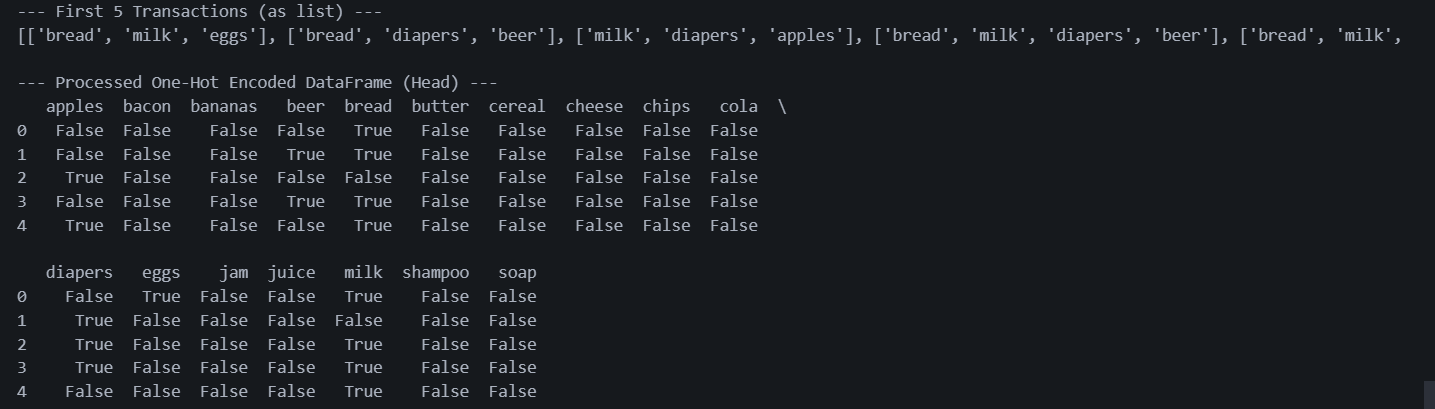
\includegraphics[width=1\textwidth]{transaction_df.png}
\caption{Output of data loading and one-hot encoding preprocessing.}
\label{fig:lab4-preprocess}
\end{figure}

Figure \ref{fig:lab4-preprocess} shows the two-step data preparation.
\begin{itemize}
    \item \textbf{First 5 Transactions:} The raw data is loaded as a list of lists, where each inner list is a customer's basket.
    \item \textbf{Processed DataFrame:} The \texttt{TransactionEncoder} successfully converts this list into a one-hot encoded DataFrame. As seen in the head, row 0 (which was `['bread', 'milk', 'eggs']`) now has `True` for the 'bread', 'milk', and 'eggs' columns, and `False` for all others. This format is required for the \texttt{mlxtend} algorithms.
\end{itemize}
\subsubsection{Run FP-Growth to Find Frequent Itemsets}
The FP-Growth algorithm is used to efficiently find itemsets that meet a minimum support threshold. A threshold of 20\% (\texttt{min\_support=0.2}) is used, meaning the itemset must appear in at least 20\% of all transactions.

\begin{lstlisting}[caption={Running FP-Growth with a minimum support of 0.2.}, label={lst:lab4-fpgrowth}]
from mlxtend.frequent_patterns import fpgrowth

frequent_itemsets_fp = fpgrowth(
    df_onehot, 
    min_support=0.2, 
    use_colnames=True
)
frequent_itemsets_fp = frequent_itemsets_fp.sort_values(
    by='support', 
    ascending=False
)
print(frequent_itemsets_fp)
\end{lstlisting}

\begin{figure}
\centering
% --- YOUR SECOND IMAGE ---
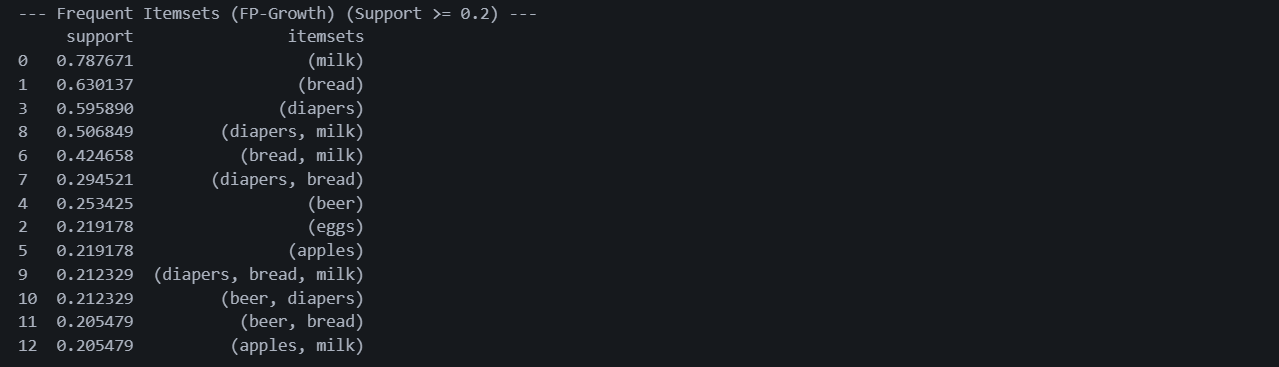
\includegraphics[width=1\textwidth]{frequent_set.png}
\caption{Frequent itemsets found by FP-Growth (min\_support >= 0.2).}
\label{fig:lab4-itemsets-fp}
\end{figure}

Figure \ref{fig:lab4-itemsets-fp} lists the 13 itemsets that appeared in at least 20\% of the 20 transactions.
\begin{itemize}
    \item \textbf{Support:} The 'support' column shows the percentage of transactions containing the itemset. For example, \texttt{(milk)} has a support of 0.787... (or 78.7\%), making it the most frequent single item.
    \item \textbf{Itemsets:} The algorithm successfully found not just single items (like \texttt{(bread)}, \texttt{(diapers)}) but also frequent multi-item sets, such as \texttt{(diapers, milk)}, \texttt{(bread, milk)}, and even the 3-item set \texttt{(diapers, bread, milk)}.
    \item \textbf{Threshold:} No itemsets with support less than 0.2 are shown, as they were pruned by the algorithm.
\end{itemize}

\subsubsection{Extract and Interpret Association Rules}
Using the frequent itemsets found by FP-Growth, we can now generate association rules. We will filter for rules that have a \textbf{confidence} of at least 60\% (\texttt{min\_threshold=0.6}). The rules are then sorted by \textbf{lift} to find the most statistically significant relationships.

\begin{lstlisting}[caption={Generating association rules from frequent itemsets.}, label={lst:lab4-rules}]
# We are filtering for rules with at least 60% confidence
rules = association_rules(
    frequent_itemsets_fp, 
    metric='confidence', 
    min_threshold=0.6
)

# Sort by 'lift' to find the most interesting rules
rules = rules.sort_values(by='lift', ascending=False)
print(rules)
\end{lstlisting}

\begin{figure}
\centering
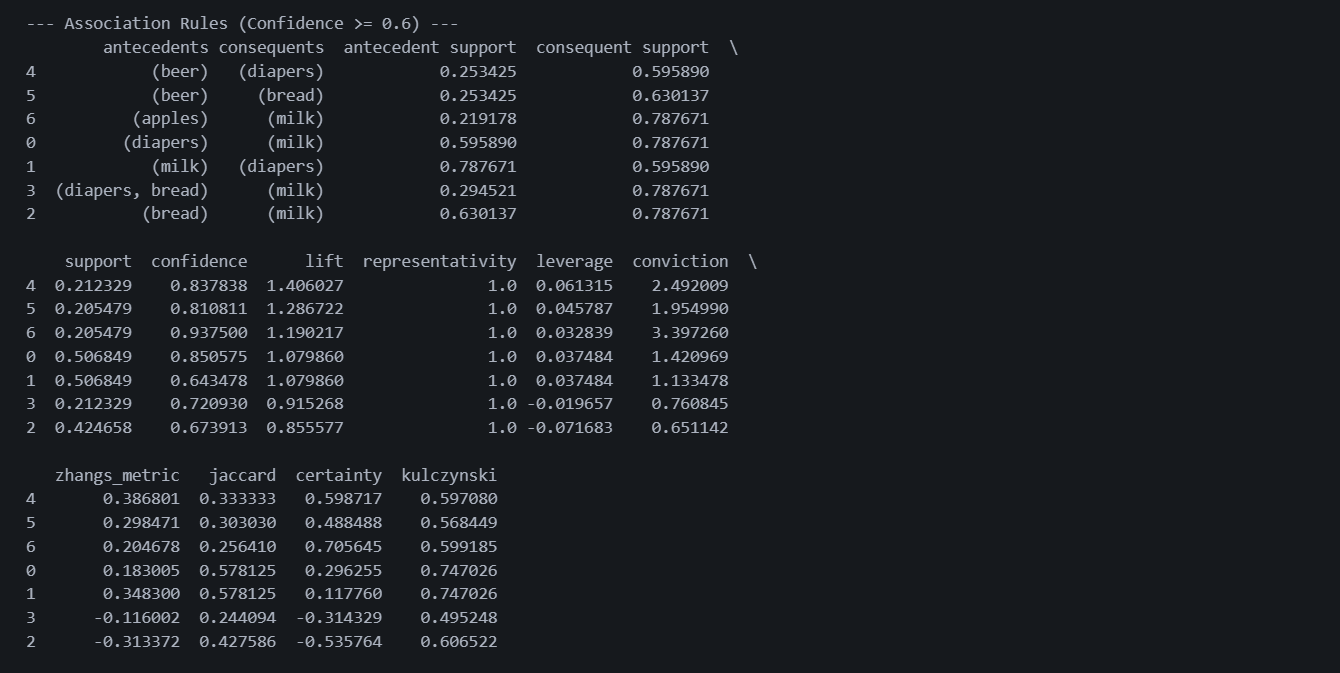
\includegraphics[width=1\textwidth]{association_rule.png}
\caption{Association rules with confidence >= 0.6, sorted by lift.}
\label{fig:lab4-rules}
\end{figure}

Figure \ref{fig:lab4-rules} displays the seven association rules that met the 60\% confidence threshold, generated by the code in Listing \ref{lst:lab4-rules}. Each row is a rule "IF \textit{antecedent} THEN \textit{consequent}".

\begin{itemize}
    \item \textbf{Confidence:} This represents the probability that a customer will buy the \textit{consequent} given that they have already bought the \textit{antecedent}. For example, in row 4, the confidence is 0.837 (83.7\%). This means that 83.7\% of customers who bought \texttt{(diapers)} also bought \texttt{(beer)}.
    
    \item \textbf{Lift:} This measures how much more likely the \textit{consequent} is purchased when the \textit{antecedent} is purchased, compared to if they were independent.
        \begin{itemize}
            \item A lift > 1 indicates a positive association (the items are likely bought together).
            \item A lift = 1 indicates no association.
            \item A lift < 1 indicates a negative association.
        \end{itemize}
    
    \item \textbf{Interpreting a Rule (Row 4):}
        \begin{itemize}
            \item \textbf{Rule:} IF `(diapers)` THEN `(beer)`.
            \item \textbf{Support (0.212):} This combination appears in 21.2\% of all transactions.
            \item \textbf{Confidence (0.837):} 83.7\% of people who bought diapers also bought beer.
            \item \textbf{Lift (1.406):} Customers are 1.4 times more likely to buy beer if they have diapers in their cart (compared to a random customer buying beer). This is the strongest positive relationship found.
        \end{itemize}
        
    \item \textbf{Interpreting a Rule (Row 2):}
        \begin{itemize}
            \item \textbf{Rule:} IF `(bread)` THEN `(milk)`.
            \item \textbf{Confidence (0.673):} 67.3\% of people who bought bread also bought milk.
            \item \textbf{Lift (0.855):} The lift is less than 1. This surprisingly indicates that while the two are bought together often, a customer who buys bread is *less* likely to buy milk than a random customer. This suggests that while both are popular, they are not a strongly linked pair.
        \end{itemize}
\end{itemize}
\section{Conclusion}
This report detailed a comprehensive data mining and machine learning project, starting from raw data and culminating in advanced modeling.

The project began with \textbf{Lab 1: Dataset Analysis}, where the data's structure and types were identified, revealing a mix of numerical and categorical features with no missing values. The target variable, \texttt{accident\_risk}, was identified as a continuous probability, framing the initial problem as a regression task.

In \textbf{Lab 2: Data Preprocessing}, the data was prepared for modeling. Missing values were artificially introduced and imputed using median and mode. Categorical features were one-hot encoded, and numerical features were standardized using Z-score scaling. Various similarity metrics (Pearson, Cosine, Euclidean, Jaccard) were computed to understand feature and sample relationships.

\textbf{Lab 3: Exploratory Data Analysis} provided key insights through visualization. Histograms revealed the distributions of all variables, notably the normal distribution of the \texttt{accident\_risk} target. Boxplots were used to identify outliers, which were found only in the \texttt{accident\_risk} column.

\textbf{Lab 4: Frequent Itemset Mining} used a different dataset to explore market basket analysis. The FP-Growth algorithm successfully extracted frequent itemsets and generated association rules, with "IF (diapers) THEN (beer)" being identified as the rule with the highest lift.

\textbf{Lab 5: Classification} converted the problem by binning the \texttt{accident\_risk} target into 'low', 'medium', and 'high' classes. A Decision Tree classifier achieved 72.0\% accuracy on a single test split and a more robust mean accuracy of 69.0\% during 10-fold cross-validation.

Finally, \textbf{Lab 6: Clustering} applied unsupervised learning. The Elbow Method and Dendrogram analysis both independently suggested an optimal cluster count of K=4. The resulting k-Means clusters were found to be well-separated, as confirmed by the PCA visualization and a good silhouette score.

Overall, this series of labs successfully demonstrated the complete data science pipeline, from data cleaning and exploration to the implementation and evaluation of supervised (Classification) and unsupervised (Clustering) machine learning models.
\end{document}